%----------------------------------------------------------------------------------------
%	PACKAGES AND THEMES
%----------------------------------------------------------------------------------------
\PassOptionsToPackage{table}{xcolor}
\documentclass[aspectratio=169,xcolor=dvipsnames,10pt]{beamer}
\usetheme{SimplePlusAIC}

\setbeamerfont{section in toc}{size=\small}

% \usepackage{background}
% \backgroundsetup{
%     placement=center,
%     scale=4,
%     % contents={Part II/logos/Simula_logo.png},
%     opacity=0.1
% }
% \setbeamertemplate{background}{\BgMaterial}

\setbeamertemplate{background}{\tikz[overlay,remember picture]\node[opacity=0.05,anchor=south west]
at (current page.south west)
{
\includegraphics[width=5cm,keepaspectratio]{Part II/logos/Simula_logo.png}};}


\useinnertheme[showtitle=false]{tcolorbox}


\usepackage{amsmath}
\usepackage{animate}
\usepackage{hyperref}
\usepackage{cleveref}
\usepackage{caption}
\usepackage{graphicx} % Allows including images
\usepackage{subfig}
\usepackage{booktabs} % Allows the use of \toprule, \midrule and  \bottomrule in tables
\usepackage{svg} %allows using svg figures
\usepackage{tikz}
\usepackage{makecell}
\usepackage{multirow}
\usepackage{appendixnumberbeamer}
\usepackage{wrapfig}
\usepackage{verbatim}
%\usepackage[dvipsnames]{xcolor}

\usepackage{hhline}
\usepackage{relsize}
\usepackage{bm}
%Select the Epilogue font (requires luaLatex or XeLaTex compilers)
%\setsansfont{Epilogue}[
  %  Path=./epilogueFont/,
  %  Scale=0.9,
  %  Extension = .ttf,
   % UprightFont=*-Regular,
   % BoldFont=*-Bold,
   % ItalicFont=*-Italic,
    %BoldItalicFont=*-BoldItalic
    %]
    \usefonttheme[onlymath]{serif}
% \usepackage{ eulervm } % Euler VM as math serif font

\newcommand*{\defeq}{\stackrel{\text{def}}{=}}
\newcommand{\grad}{\nabla}
\newcommand{\lap}{\Delta}
\newcommand{\weaklyto}{\rightharpoonup}
\newcommand{\weakstar}{\stackrel{*}\rightharpoonup}
\newcommand{\cts}{\hookrightarrow}
\newcommand{\ctsDense}{\xhookrightarrow{d}}
\newcommand{\ctsCompact}{\xhookrightarrow{c}}
\newcommand{\E}{\mathbb{E}}
\newcommand{\bE}{\mathbb{E}}
\newcommand{\fF}{\mathfrak{F}}
\newcommand{\pP}{\mathbb{P}}
\newcommand{\bP}{\mathbb{P}}
\newcommand{\cP}{\mathcal{P}}
\newcommand{\R}{\mathbb{R}}
\newcommand{\bR}{\mathbb{R}}
\newcommand{\ER}{\overline{\mathbb{R}}}
\newcommand{\cR}{\mathcal{R}}
\newcommand{\cJ}{\mathcal{J}}
\newcommand{\cG}{\mathcal{G}}
\newcommand{\CVaR}{\textup{CVaR}}
\newcommand{\D}{\textup{ d}}
\newcommand{\dd}{\mathrm{d}}
\newcommand{\fa}{\text{for all }}
\DeclareMathOperator*{\essinf}{\vphantom{p}ess\,inf}
\DeclareMathOperator{\sigmoid}{expit} % a.k.a. logistic sigmoid

\newtheorem{proposition}{Proposition}

\usepackage[ruled,vlined,algo2e]{algorithm2e}
\crefname{algocf}{algorithm}{algorithms}
 \usepackage{caption}

%----------------------------------------------------------------------------------------
%	TITLE PAGE
%----------------------------------------------------------------------------------------



\title[Intro to OUU]{An Introduction to Optimization under Uncertainty II: Stability, Algorithms, and Computational Statistics 
 } % The short title appears at the bottom of every slide, the full title is only on the title page
%\subtitle{Subtitle}

\author{\small{\bf Thomas M. Surowiec}}

\institute[SCAN, Simula]{Department of Numerical Analysis and Scientific Computing \newline Simula Research Laboratory \newline Oslo, Norway}
% Your institution as it will appear on the bottom of every slide, maybe shorthand to save space


\date[NUMRAD 2024\\ June 12, 2024]{ {\footnotesize 
NUMRAD 2024, June 12, 2024}}
%----------------------------------------------------------------------------------------
%	PRESENTATION SLIDES
%----------------------------------------------------------------------------------------



\begin{document}
{
\setbeamertemplate{background canvas}{}
\frame{\titlepage}
}

\begin{frame}{Overview}
\tableofcontents
\end{frame}

\section{Stability}
\subsection{Stability of Solutions and Optimal Values}
\begin{frame}{Statistical Numerical Analysis}
\begin{exampleblock}{}
    \begin{itemize}
        \visible<1->{
         \item Are solutions and optimal values \alert{stable} with respect to \alert{shifts in distribution}?
        \item Can this stability be quantified?
        \item What happens \alert{asymptotically} in the "big data" limit?
        }
    \end{itemize}
\end{exampleblock}

    \begin{exampleblock}{}
        \visible<2->{
        \begin{center}
        \textit{These are \alert{fundamentally different} questions to traditional numerical analysis in PDEs and optimal control:}
    \end{center}
        }
    \end{exampleblock}

    \begin{exampleblock}{}
    \begin{itemize}
        \item \visible<3->{In the FEM, the solution spaces are replaced by finite dimensional function spaces, but the measure remains the Lebesgue measure.
        \item Mesh refinement obviously increases the dimension of these spaces, but refinements are (typically) not random.}
    \end{itemize}
    \end{exampleblock}
\end{frame}

\begin{frame}\frametitle{What do we mean by ``stability''?}

\begin{exampleblock}{A News Vendor Problem (see e.g. Shapiro, Dentcheva, Ruszczynski (2009))}
\begin{itemize}
\item \visible<2->{ How much to order of $x$ (deterministic) to satisfy demand $d$ (stochastic)?
\item Cost: $c > 0$ per unit
\item Additional: Backorder cost $b > c$, holding cost $h \ge 0$ per unit.
\item A stochastic optimization problem:
\[
\min_{x \ge 0} \{ f(x) := \mathbb E_{\xi}[ cx + b \max\{0,d(\xi)-x\} + h\max\{0,x-d(\xi)]\}\}
\]
\item ``Maximize (avg.) performance of $x$ by minimizing expected cost.''
}
\item \visible<3->{Assume $d \sim U(1,2)$.  Then 
\[
x^{\star} = H^{-1}(\kappa) = 1 + \kappa \text{ where } \kappa = \frac{b - c}{b + h}\quad \text{($H^{-1}$ is the quantile function for $d$)}
\]
}\vspace{-2ex}
\end{itemize}
\end{exampleblock}
\end{frame}

\begin{frame}\frametitle{What do we mean by ``stability''?}
\begin{exampleblock}{A News Vendor Problem (see e.g. Shapiro, Dentcheva, Ruszczynski (2009))}
\begin{itemize}
\item \visible<1->{What if the distribution of $d$ is \textbf{not known} or \textbf{estimated from data}?
}
\item \visible<2->{Given: $d_{1},\dots, d_{N}$ (scenarios) with probabilities $p_{1}, \dots, p_{N}$. 
\item We must consider instead:
\[
\min_{x \ge 0} \{ \widehat{f}_{N}(x) :=  \sum_{i=1}^{N} p_i (cx + b \max\{0,d_i-x\} + h\max\{0,x-d_i\} )\}
\]
%\item This is now a nonsmooth optimization problem!
\item Continuous case: $b = 2, c = 1, h = 1 \Rightarrow x^{\star} = 4/3$
\item Does the solution of the discrete problem $\widehat{x}^{\star}_N$ approach $4/3$ as $N \to +\infty?$ }
\end{itemize}
\end{exampleblock}
\end{frame}

\begin{frame}\frametitle{What do we mean by ``stability''?}
\begin{exampleblock}{}
\begin{itemize}
\item Q: Does $\widehat{x}^{\star}_N \to x^{\star} = 4/3$ as $N \to +\infty?$ 
\item A: \textbf{Yes, slowly}$^*$.\vspace{-3ex}
\end{itemize}
\begin{figure}
%  \centering
    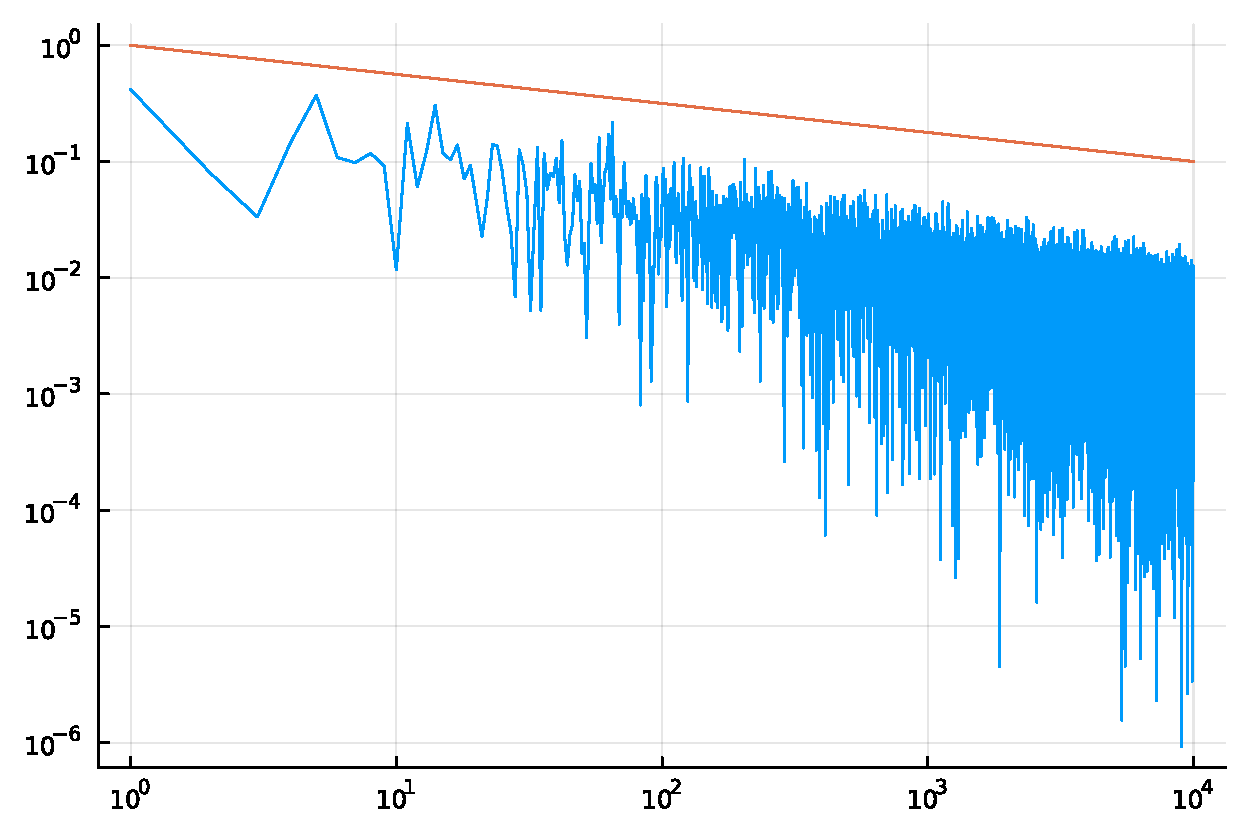
\includegraphics[width = 0.4\textwidth,keepaspectratio]{figures/EmpiricalStability1D.pdf}
      \caption{\footnotesize Sample size $N$ versus error $|x^{\star} - \widehat{x}^{\star}_{N}|$ (blue line), $N^{-1/4}$ (orange line). $*:$ $\widehat{x}^{\star}_N$ calculated for each $N$ via projected subgradients with fixed step size $0.075$ up to max 100 iterations.}
\end{figure}\vspace{-3ex}
\end{exampleblock}
% {\tiny
% $*:$ $\widehat{x}^{\star}_N$ calculated for each $N$ via projected subgradients with fixed step size $0.075$ up to max 100 iterations.
% }
\end{frame}

\begin{frame}{Defining Stability in OUU}
\vspace{-1ex}
\begin{exampleblock}{}
\begin{equation*}%\label{eq:nu_of_p}
\aligned
&\text{Optimal Value:}  &\nu(P) &= \inf_{z \in \mathcal{Z}_{\rm ad}} \int_{\Omega} f(z,\omega) \ \mathrm{d}P(\omega).\\
&\text{Optimal Solutions:}  &z(P) &\in \mathop{\mathrm{argmin}}_{z \in \mathcal{Z}_{\rm ad}} \int_{\Omega} f(z,\omega) \ \mathrm{d}P(\omega)
\endaligned
\end{equation*}
\end{exampleblock}
\vspace{-1ex}
\begin{exampleblock}{}
\begin{itemize}
\item \visible<1->{If $P$ is replaced by $P_{N}$ such that $P_{N} \Rightarrow P$, does it hold that 
\[ 
\nu(P_{N}) \to \nu(P)\text{ and } \| z(P_N) - z(P) \|_{\mathcal{Z}} \to 0?
\]} \vspace{-4ex}
\item \visible<2->{If so, can we quantify this convergence somehow?}
\item \visible<3->{What if we have to replace $\mathcal{Z}$ by $\mathcal{Z}_{h}$ with $\mathrm{dim}\, \mathcal{Z}_h < +\infty$ in practice? Does it hold that 
\[ 
\nu^{h}(P_{N}) \to \nu(P)\text{ and } \| z^h(P_N) - z(P) \|_{\mathcal{Z}} \to 0 \text{ as $h \to 0$ and $N \to +\infty$?}
\]
}
\end{itemize}
\end{exampleblock}
\end{frame}
    
\begin{frame}\frametitle{A (Very) Brief History}
\begin{exampleblock}{}
{\smaller
\textbf{Qualitative} and \textbf{quantitative stability analysis} has been developed for \textbf{$n$-dimensional parameter spaces} $\Theta$ and nontrivial constraint sets since at least the 1980s:
\begin{itemize}
\item  Wets 1979, Solis \& Wets 1981, 1983
\item  Dupa\v{c}ov\'a 1983a, 1983b, 1984a, 1984b, 1987; 
\item Dupa\v{c}ov\'a \& Wets 1986, 1988
\end{itemize}
As noted in Dupa\v{c}ov\'a \& Wets 1988, ``\textit{there is substantial statistical literature dealing with the questions broached here}'' notably
\begin{itemize}
\item Wald 1949,
% A. WALD, "Note on the consistency of the maximum likelihood estimate," Ann. Math.
% Statist., Vol. 20 (1949), pp. 595-601.
\item Huber 1967
% VOL. 5.1 | 1967
% The behavior of maximum likelihood estimates under nonstandard conditions
% Peter J. Huber 
% Berkeley Symp. on Math. Statist. and Prob., 1967: 221-233 (1967)
\end{itemize}
(the latter exclude constraints, require smoothness, ... )\medskip

\begin{itemize}
\item See also the (many) contributions and book chapters by Shapiro 2003, Pflug 2003.
% https://doi.org/10.1016/S0927-0507(03)10006-0
% https://doi.org/10.1016/S0927-0507(03)10007-2
\item Our perspective  is based  largely on \alert{Rachev \& R\"omisch 2002}.
% Svetlozar T. Rachev, Werner Römisch, (2002) Quantitative Stability in Stochastic Programming: The Method of Probability Metrics. Mathematics of Operations Research 27(4):792-818.
% https://doi.org/10.1287/moor.27.4.792.304
\item None of this work has been developed for $\infty$-dim. stochastic optimization
\end{itemize}
}
\end{exampleblock}
\end{frame}

\begin{frame}{Linear Quadratic Risk-Neutral Problems}
    \begin{exampleblock}{}
\begin{itemize}
\item $D \subset \mathbb R^m$ open, bounded domain, $\partial D$ is Lipschitz.
\item $V = H^1_0(D)$ with inner product $(u,v)_{V} = (\nabla u, \nabla v)_{L^2(D)}$.
\item $V^* =  H^{-1}(D)$ topological dual of $V$ with dual pairing $\langle\cdot,\cdot\rangle$.
\item $H = L^2(D)$ with inner product $(u,v)_{H}$.
\item $\Xi$ is a metric space, $P \in \mathcal{P}(\Xi)$ the set of all Borel probability measures.
\end{itemize}
\end{exampleblock}
\end{frame}

\begin{frame}\frametitle{Linear Quadratic Risk-Neutral Problems}
\begin{exampleblock}{}
\begin{itemize}
\item Consider the bilinear form 
$a(\cdot,\cdot;\xi): V \times V\to\mathbb R$ defined by
\[
\textcolor{Black}{
a(u,v;\xi)=\int_{D}\sum_{i,j=1}^{n}a_{ij}(x,\xi)\frac{\partial u(x)}{\partial x_{i}}
\frac{\partial v(x)}{\partial x_{j}}\mathrm{d}x\quad(\xi\in\Xi).}
\]
\item $a_{ij}:D\times\Xi\to\mathbb R$ are  measurable on $D\times\Xi$ and there exist $L>\gamma>0$:
\[
\textcolor{Black}{
\gamma
\sum_{i=1}^{n}y_{i}^{2}
\le
\sum_{i,j=1}^{n}a_{ij}(x,\xi)y_iy_j
\le 
L\sum_{i=1}^{n}y_{i}^{2}\quad(\forall y\in\mathbb R^{n})}
\]
for a.e. $x\in D$ and $P$-a.e. $\xi\in\Xi$. (i.e, each $a_{ij}$ is essentially bounded.) 
\end{itemize}
\end{exampleblock}
\end{frame}

\begin{frame}\frametitle{Linear Quadratic Risk-Neutral Problems}
\begin{exampleblock}{}
\begin{itemize}
\item \textcolor{Black}{Minimize} the functional
 \textcolor{Black}{
 \begin{eqnarray*}
 {\mathcal{J}}(u,z) \!
 &:=& \frac{1}{2} \bE_{\bP}[\| u - \widetilde{u}_d \|^2_{H}] + 
 \frac{\alpha}{2} \| z \|^2_{H}
 \end{eqnarray*}}\\ \vspace{-2ex}
 subject to \textcolor{Black}{$z\in \mathcal{Z}_{\rm ad} \subset H$} (a closed convex bounded set), where 
  \textcolor{Black}{$u$ satisfies}
\[
\textcolor{Black}{a(u,v;\xi)=\int_{D}(z(x)+g(x,\xi))v(x)dx 
\quad\mbox{for }\bP \mbox{-a.e. }\xi\in\Xi}, 
\]
for all test functions $v\in C_{0}^{\infty}(D)$. 
\item We also assume
% \begin{itemize}
% \item 
\textcolor{Black}{ $\alpha>0$}, 
% \item 
\textcolor{Black}{$\widetilde{u}_{d}\in H$}, 
% \item 
\textcolor{Black}{$g:D\times\Xi\to\bR$} is measurable and (at least) $L^2$ in $D$.
% \end{itemize}
\end{itemize}
\end{exampleblock}
\end{frame}

\begin{frame}{Linear Quadratic Risk-Neutral Problems}
    \begin{exampleblock}{}
\centering 
\visible<1->{We derive a class of integrands $f : \mathcal{Z} \times \Xi \to \mathbb R$ to motivate the general framework.}
\end{exampleblock}

\visible<2->{
\begin{exampleblock}{}
\begin{itemize}
\item For each $\xi\in\Xi$ define $A(\xi):V\to V^{\star}$ 
via the Riesz Representation Thm:
\[
\textcolor{Black}{\langle A(\xi)u,v \rangle = a(u,v;\xi)
\quad(u,v\in V)}.
\]
\item \textcolor{Black}{$A(\xi)$ is  linear, uniformly 
positive definite (with $\gamma>0$) and uniformly bounded 
(with $L>0$)} 
\item The random PDE may be written in the form
\[
\textcolor{Black}{A(\xi)u=z+g(\xi)\quad(\bP\mbox{-a.e. }\xi\in\Xi).}
\]
 \end{itemize}
\end{exampleblock}
}
\end{frame}

\begin{frame}\frametitle{Linear Quadratic Risk-Neutral Problems}
\begin{exampleblock}{}
\centering 
We derive a class of integrands $f : \mathcal{Z} \times \Xi \to \mathbb R$ to motivate the general framework.
\end{exampleblock}
\begin{exampleblock}{}
\begin{itemize}
\item \visible<2->{\textcolor{Black}{$A(\xi)^{-1}:V^{\star}\to V$ exists and is positive  definite (with $\frac{1}{L}$) and bounded (with $\frac{1}{\gamma}$)}.
}
\item \visible<3->{
We consider 
the integrand
\begin{eqnarray*}
\textcolor{Black}{f(z,\xi)}%&=&
%\frac12\big\|A(\xi)^{-1}(z+g(\xi))-
%\widetilde{u}_{d}\big\|_{H}^{2}+\frac{\alpha}{2}\|z\|_{H}^{2}\\
%&=&\textcolor{Blue}{\frac{1}{2}\big\|A(\xi)^{-1}z -
%(\widetilde{u}_{d}-A(\xi)^{-1}g(\xi))\big\|_{H}^{2}+
%\frac{\alpha}{2}\|z\|_{H}^{2}}\\
&=&\textcolor{Black}{\frac{1}{2}\big\|A(\xi)^{-1}z -
\widetilde{u}_{d}(\xi)\big\|_{H}^{2}+
\frac{\alpha}{2}\|z\|_{H}^{2}}
\end{eqnarray*}
for any $z\in \mathcal{Z}_{\rm ad}$ and $\xi\in\Xi$,
\item  This provides us with an 
\textcolor{Black}{$\infty$-dimensional stochastic 
optimization problem}:
\begin{equation}\label{sopde}
\textcolor{Black}{\min\left\{F_{\bP}(z)=\int_{\Xi}f(z,\xi)\mathrm{d}\bP(\xi): 
z\in \mathcal{Z}_{\rm ad}\right\}}.
\end{equation}
}
\end{itemize} 
\end{exampleblock}
\end{frame}

\begin{frame}{Theoretical Properties}
\begin{proposition}[Hoffhues, R\"omisch, Surowiec (2021)]\label{p1}
\visible<1->{For each $P\in\cP(\Xi)$ the functional $F_{P}$ is finite, 
continuous, and strongly convex on $H$ and, hence, weakly 
lower semicontinuous on the weakly compact set $\mathcal{Z}_{\rm ad}$.}%
\visible<2->{
Moreover, there exists an unique minimizer $z(P)\in 
\mathcal{Z}_{\rm ad}$ of \eqref{sopde} and the objective function 
$F_{P}$ has quadratic growth around $z(P)$, i.e. we have
\begin{equation}\label{quadrgrowth}
\|z-z(P)\|_{H}^{2}\leq\frac{8}{\alpha}(F_{P}(z)-F_{P}(z(P)))
=\frac{8}{\alpha}(F_{P}(z)-v(P))\quad(\forall z\in 
\mathcal{Z}_{\rm ad}).
\end{equation}
}\visible<3->{In addition, $F_{P}$ is G\^ateaux differentiable on $H$
with G\^ateaux derivative $F'_{P}(\cdot)$ and the estimate
\begin{equation}\label{Gdiff}
|F_{P}(z)-F_{P}(\tilde{z})|\le\sup_{t\in[0,1]}
\|F'_{P}(z+t(\tilde{z}-z))\|\,\|z-\tilde{z}\|_{H}
\end{equation}
holds for all $z,\tilde{z}\in H$.
}
\end{proposition}
\end{frame}

\begin{frame}{Possible Generalizations}
\begin{exampleblock}{}
\begin{itemize}
    \item The previous result is for a rather specific case.
    \item The essential part for stability analysis is the \alert{growth condition}, which is heavily dependent on the strong convexity of $F_{P}$.
    \item In general, we need a continuous bijection $\phi:\mathbb R_+ \to \mathbb R_+$ such that
    \[
    \phi(\|z-z(P)\|_{H})\leq F_{P}(z)-F_{P}(z(P))
    \]
    (This will be clear in a moment.)
    \item The local Lipschitz bound \eqref{Gdiff} is also clearly available for more general objective functions.
\end{itemize}
\end{exampleblock}
\end{frame}

\begin{frame}\frametitle{Quantifying Stability}
\begin{exampleblock}{}
Q:
How can we \alert{quantify} results like:
\[ 
\nu(P_{N}) \to \nu( P)\text{ and } \| z(P_N) - z(P) \|_{\mathcal{Z}} \to 0?
\]
A: Probability metrics.
\end{exampleblock}
\end{frame}
\begin{frame}\frametitle{Probability Metrics}
\visible<1->{
\begin{exampleblock}{}
\centering
But how can we measure the distance between probability measures?
\end{exampleblock}
}
\vspace{-1ex}
\visible<2->
{\begin{exampleblock}{}
\begin{itemize}
\item $\Xi$ a metric space, $\left\{P_{N}\right\} \subset \mathcal{P}(\Xi)$.
\item $P_N$ converges weakly to $P$ in $\mathcal{P}(\Xi)$ iff 
\[
\textcolor{Black}{
\lim_{N \to \infty} \mathbb E_{P_{N}}[f] 
= 
\lim_{N\to\infty}\int_{\Xi}f(\xi)\mathrm{d} \bP_{N}(\xi) 
=
\int_{\Xi}f(\xi)\mathrm{d} \bP(\xi) 
=
\mathbb E_{P}[f].
}
\]
for all bounded continuous functions $f \in C_{b}(\Xi,\bR)$.
\item The topology of weak convergence is \textbf{metrizable} if $\Xi$ is separable.
\end{itemize}
\end{exampleblock}
}
\end{frame}

\begin{frame}\frametitle{Zolotarev's $\zeta$-distances}
\begin{exampleblock}{}
Zolotarev {\color{Black}$\zeta$-distance} on $\mathcal{P}(\Xi)$ (Zolotarev 83):
\[
\textcolor{Black}{d_{\mathfrak F}(\bP,\mathbb Q)=\sup_{f  \in \mathfrak F}\left|
\int_{\Xi}f(\xi)\mathrm{d}\bP(\xi) - \int_{\Xi}f(\xi)
\mathrm{d} \mathbb Q(\xi)\right|},
\]
where $\mathfrak F$ is a family of real-valued Borel measurable 
functions on $\Xi$.
% @article{Zolotarev1984,
%   title = {Probability Metrics},
%   volume = {28},
%   ISSN = {1095-7219},
%   url = {http://dx.doi.org/10.1137/1128025},
%   DOI = {10.1137/1128025},
%   number = {2},
%   journal = {Theory of Probability &amp; Its Applications},
%   publisher = {Society for Industrial & Applied Mathematics (SIAM)},
%   author = {Zolotarev,  V. M.},
%   year = {1984},
%   month = jan,
%   pages = {278–302}
% }
\end{exampleblock}\vspace{-1ex}
\begin{exampleblock}{}
\centering
Whether convergence wrt $d_{\mathfrak F}$ implies or 
is implied by weak convergence depends on the richness and 
on analytical properties of $\mathfrak F$.
\end{exampleblock}
\end{frame}

\begin{frame}\frametitle{Probability Metrics}
\begin{exampleblock}{}
\centering
The right tool for the right job...
\end{exampleblock}

\begin{exampleblock}{}
A number of important probability metrics are of the form $d_{\mathfrak F}$:
\begin{itemize}
\item \textcolor{Blue}{bounded Lipschitz metric} (metrizes top'y of weak convergence) 
\item \textcolor{Blue}{Fortet-Mourier type metrics}: \pause For $p \in [1,\infty)$, let $\mathfrak F = \mathcal{F}_p(\Omega)$, where ($d$ metric on $\Omega$)
\begin{multline*}
\hspace{-2ex}\mathcal{F}_{p}(\Omega) := \left\{ f : \Omega \to \mathbb R \left|\;\right.\right. 
| f(\omega_1) - f(\omega_2)| \le\\ \left.\max\{1,d(\omega_1,\omega_0)^{p-1}, d(\omega_2,\omega_0)^{p-1}\}d(\omega_1,\omega_2) \quad \forall \omega_1,\omega_2 \in \Omega \right\},
\end{multline*}
\item \pause Rachev (1991): $\mathbb P_N \to \mathbb P$ weakly in $\mathcal{P}(\Omega)$ iff $d_{\mathcal{F}_p(\Omega)}(\mathbb P_N,\mathbb P) \to 0$. \pause
\item Why not \textcolor{Blue}{Wasserstein}? \vspace{-2ex}
% \begin{multline*}%\label{eq:fortet_mourier_wasserstein_p}
\[
\hspace{-7.5ex}d_{\mathcal{F}_p(\Omega)}(\mathbb P,\mathbb Q) 
\le \left(1 + \int_{\Omega} d(\omega_0,\omega)^p \ \mathrm{d} \mathbb P(\omega) + \int_{\Omega} d(\omega_0,\omega)^p \ \mathrm{d}\mathbb Q(\omega)\right)^{\frac{p-1}{p}} W_p(\mathbb P,\mathbb Q)
\]
\end{itemize}
\end{exampleblock}
\end{frame}

\begin{frame}\frametitle{Probability Metrics}
\visible<1->{
\begin{lemma}[Tops{\o}e (1967)]
Let  $\fF$ be uniformly bounded and $\bP(\{\xi\in\Xi:\fF\mbox{ 
is not equicontinuous at }\xi\})=0$\footnote{\tiny
$\fF$ is equicontinuous at $\xi_0 \in \Xi$ if
$(\forall \epsilon > 0, \exists \delta > 0 : f \in \fF$, $\xi \in \Xi, d(\xi_0,\xi) < \delta \Rightarrow |f(\xi_0) - f(\xi)| < \epsilon$)
} holds. Then 
\textcolor{Blue}{$\fF$ is a $\bP$-uniformity class, i.e., 
weak convergence of $(\bP_{N})$ to $\bP$ implies} 
\[
\lim_{N\to\infty}d_{\fF}(\bP_{N},\bP)=0.
\]
\end{lemma}
}
\visible<2->{
\begin{exampleblock}{}
\begin{itemize}
\item Compared with classical probability metrics we consider a 
much smaller family $\fF$:
\[
\textcolor{Blue}{\fF_{\rm mi}=\{f(z,\cdot):z\in \mathcal{Z}_{\rm ad}\} \quad \text{(minimal information (m.i.) family)}}. 
\]
\item This leads to a \textcolor{Blue}{pseudometric}:
the \textcolor{Blue}{minimal 
information (m.i.) distance} $d_{\fF_{\rm mi}}$.
\end{itemize}
\end{exampleblock}
}
\end{frame}

\begin{frame}{Properties of $\fF_{mi}$}
    \begin{theorem}[Hoffhues, R\"omisch, Surowiec (2021)]\label{t2}
    Assume that
    \begin{enumerate}
        \item for all $i,j=1,\ldots,m$ each $a_{ij}(x,\cdot) : \Xi \to \mathbb R$ is Lip\-schitz 
         uniformly with respect to $x\in D$,
\item $g(x,\cdot):\Xi \to \mathbb R$ is Lip\-schitz uniformly with respect to $x\in D$,
\item $g\in L^{\infty}(\Xi,\mathcal{B},P;H)$.
    \end{enumerate}
    Then the minimal information family $\fF_{mi}=\{f(z,\cdot):z\in Z_{\rm ad}\}$ is
    \begin{enumerate}
        \item uniformly bounded,
        \item Lipschitz continuous. 
    \end{enumerate}
In particular, \alert{$\fF_{mi}$ is a $P$-uniformity class.}
\end{theorem}
\end{frame}

\begin{frame}\frametitle{Lipschitz-type Estimates for $d_{\fF_{\rm mi}}$}
\begin{theorem}[Hoffhues, R\"omisch, Surowiec (2021)]\label{t1}
Under the standing assumptions we obtain the estimates 
\begin{eqnarray}\label{infstab}
|v(Q)-v(P)|&\leq& d_{\fF_{mi}}(P,Q)\\
\only<1>{\|z(Q) - z(P)\|_{H}&\leq& 2\sqrt{\frac{2}{\alpha}}
d_{\fF_{mi}}(P,Q)^{\frac12}}
\only<2>{\alert{
\|z(Q) - z(P)\|_{H}}&\alert{\leq}& \alert{\phi^{-1}(
d_{\fF_{mi}}(P,Q))\quad \text{(recall growth condition, pg 27)}
}
}
\label{solstab}
\end{eqnarray}
for the optimal value $v(P)$ and solution $z(P)$ of
\eqref{sopde} if the original probability distribution 
$P$ is perturbed by any $Q\in\cP(\Xi)$.
\end{theorem}
\begin{exampleblock}{}
\centering This quantifies changes in optimal value and solution under \alert{shifts in the underlying distribution.}
\end{exampleblock}
\end{frame}



\begin{frame}{A Refined Estimate}
\visible<1->{
    \begin{theorem}[R\"omisch, Surowiec (2023)]\label{t3}
Under the standing assumptions the Lipschitz-type estimate
\begin{equation}\label{Lipest}
\|z(Q)-z(P)\|_{H}\leq\frac{8}{\alpha}d_{\fF_{di}}(P,Q)
\end{equation}
holds for all $P,Q\in\cP(\Xi)$, where $\fF_{di}$ 
denotes the following function class on $\Xi$
\begin{equation}\label{derivintegr}
\fF_{di}=\left\{\langle A(\cdot)^{-1}(z+g(\cdot))-
\tilde{u},A(\cdot)^{-1}h\rangle_{H}+\alpha\langle 
z,h\rangle_{H}:z\in Z_{\rm ad},\|h\|_{H}\le 1\right\}.
\end{equation}
\end{theorem}
}
\visible<2->{
\begin{exampleblock}{}
Without quadratic growth, we need the existence of a continuous monotone bijection $\widehat{\phi}:\mathbb R_+ \to \mathbb R_+$ that satisfies
\[
\phi(\|z - y\|) \ge \widehat{\phi}(\|z-y\|)\|z-y\|
\]
to generalize this bound to $\|z(Q) - z(P)\|_{H} \le \widehat{\phi}^{-1}(d_{\fF_{di}}(P,Q))$.
\end{exampleblock}
}
\end{frame}

\subsection{Monte Carlo Approximation}
\begin{frame}{Empirical Approximation}
\begin{exampleblock}{}
    \begin{itemize}
        \item $\xi_1,\xi_2,\ldots,\xi_n,\ldots$ independent 
identically distributed (iid) $\Xi$-valued random 
variables on a complete probability space 
$(\Omega,\mathcal{F},\bP)$ with the common distribution $P$ i.e., $P=\bP\circ \xi_1^{-1}$. 
        \item $\delta_{\xi}$ denotes the Dirac measure, which
places mass $1$ at $\xi\in\Xi$ and mass $0$ elsewhere
        \item The empirical probability measure:
\begin{equation}\label{empmeas}
P_n(\cdot)=\frac{1}{n}\sum_{i=1}^n\delta_{\xi_i(\cdot)}
\quad(n\in\mathbb N),
\end{equation}
\item For a random sample of size $n$, $P_n(\cdot)$ acts as a \alert{perturbation of $P$}.
    \end{itemize}
\end{exampleblock}
\pause
\begin{exampleblock}{}
\begin{itemize}
    \item $(P_{n}(\cdot)) \Rightarrow P$ $\mathbb P$-almost surely.
    \item Since $\fF_{mi}$, $\fF_{di}$ are $P$-uniformity classes, we have
    \[
    v(P_{n}(\cdot)) \to v(P) \text{ and } z(P_{n}(\cdot)) \to z(P) \qquad \bP\text{-a.s.}
    \]
\end{itemize}
\end{exampleblock}
\end{frame}

\begin{frame}\frametitle{Rate of Convergence and CLT}
\begin{theorem}[R\"omisch, Surowiec (2023)]\label{t5}
Assume that
\begin{enumerate}
    \item $\Xi\subset\mathbb R^d$ is bounded, convex set and $\Xi\subseteq{\rm cl}\;{\rm int}\,\Xi$,
    \item $k\in\mathbb N$ satisfies $d<2k$,
    \item for all $i,j=1,\ldots,m$, $a_{ij}(x,\cdot):\Xi\to\mathbb R$ and $g(x,\cdot):\Xi\to\mathbb R$ have continuous partial derivatives up to order $k$, which are all measurable and essentially bounded on $D\times\Xi$.
\end{enumerate}
Then
\begin{enumerate}
    \item $\mathbb E_{\mathbb P}[|v(P_{n}(\cdot))-v(P)|] = O(n^{-\frac12})$,
    \item $\mathbb E_{\mathbb P}[\|z(P_{n}(\cdot))-z(P)\|_{H}] = O(n^{-\frac12})$,
    \item  $(\sqrt{n}(v(P_n(\cdot))-v(P))) \rightsquigarrow \mathcal{N}(0,P(f(z(P)))^{2})$
\end{enumerate}
\end{theorem}    
\end{frame}

\begin{frame}\frametitle{Remarks}
\begin{exampleblock}{}
    \begin{itemize}
        \item The $O(n^{-\frac{1}{2}})$ convergence rates for Monte Carlo approximations can be derived without the smoothness assumptions (J. Milz ()) by looking at tail estimates for a slightly more general case than here. 
%         @article{Milz2022,
%   title = {Sample average approximations of strongly convex stochastic programs in Hilbert spaces},
%   volume = {17},
%   ISSN = {1862-4480},
%   url = {http://dx.doi.org/10.1007/s11590-022-01888-4},
%   DOI = {10.1007/s11590-022-01888-4},
%   number = {2},
%   journal = {Optimization Letters},
%   publisher = {Springer Science and Business Media LLC},
%   author = {Milz,  Johannes},
%   year = {2022},
%   month = may,
%   pages = {471–492}
% }
        \item The general stability results and central limit theorem, however, requires us to use empirical process theory.
        \item This requires knowledge of so-called metric entropy numbers; smoothness in $\xi$ related to dimension $d$ is essential.
        \item The boundedness assumptions on $\Xi$ can be relaxed.
    \end{itemize}
\end{exampleblock}\pause
\begin{exampleblock}{}
    \centering
    How do these results manifest in practice?
\end{exampleblock}
\end{frame}


\section{The Semismooth Newton Method}
\subsection{Example}
\begin{frame}{A Random Elliptic Operator}
\begin{exampleblock}{}
    \begin{itemize}
        \item \visible<1->{$D = (0,1)^2$, $\Xi = [0,1]^d$, where
$d = 2^q$, $q \in \mathbb N_0$}
        \item \visible<2->{$[0,1]$ split into $d$ intervals $D_i$ ($i = 1,\dots,d$) of the form
$
D_i = [i / d, (i + 1) / d]
$} 
        \item \visible<3->{$\chi_{i}$ is the characteristic function, 
i.e., $\chi_{i}(x)$ is $1$ if $x \in D_i$ and $0$ otherwise.}\medskip

        \item \visible<4->{$\hat{a}(x,\eta) := \sum_{i=1}^d (\eta_i + 10^{-2}x_2+10^{-3})\chi_{i}(x_1)$ $x \in D$ and $\eta \in \mathbb R^d$}\medskip

        \item \visible<5->{$(w_k(\xi))_j := (\xi_j - 10^{-1} )^k  \max\{0,\xi_j - 10^{-1} \}$ $k \in \mathbb N_0$, $ j = 1,\dots,d$, $\xi \in \Xi \subset \mathbb R^d$
        }\medskip 
        
        \item \visible<6->{$a_k(x,\xi) = \hat{a}(x,w_k(\xi))$, $a_{ij}(x,\xi) = a_k(x,\xi)$ for $k \in \mathbb N_0$, every $i,j$.
        }\medskip

        \item \visible<7->{$k = 0$ implies $a_k(x,\cdot)$ is only Lipschitz, otherwise $a_k(x,\cdot)$ is in $C^k(\Xi)$.}\medskip

        \item \visible<8->{
        We define the bilinear form
$
a_k(u,v;\xi) = \int_{D} a_k(x,\xi) \nabla u \cdot \nabla v\, \mathrm{d} x,
$
where $u,v \in H^1_0(D)$, $\xi \in \Xi$.
        }
    \end{itemize}
\end{exampleblock}
\end{frame}

\begin{frame}{A Random Elliptic PDE}
    \begin{exampleblock}{}
        \begin{itemize}
            \item \visible<1->{For the right hand side:
            $g(x,\nu) = \sin(2 x_1) \sin(2x_2) + 10^{-2}\nu$, $(x,y) \in \Omega$, $\nu \in \mathbb R$. $\nu$ is understood to be part of the vector $\xi$ and $\Xi$ will be henceforth a subset of $\mathbb R^{d+1}$
            }

            \item \visible<2->{
            $z \in L^2(\Omega)$, we then define the random elliptic PDE :
\begin{equation}\label{eq:rand_pde}
a_k(u(\xi),v;\xi) = \int_{D}(z(x) + g(x,\xi))v\, dx, \quad \text{ $u(\xi),v \in H^1_0(\Omega)$. }
\end{equation}
            }
        \end{itemize}

\end{exampleblock}
\vspace{-2ex}
\visible<3->{
\begin{figure}
  \subfloat{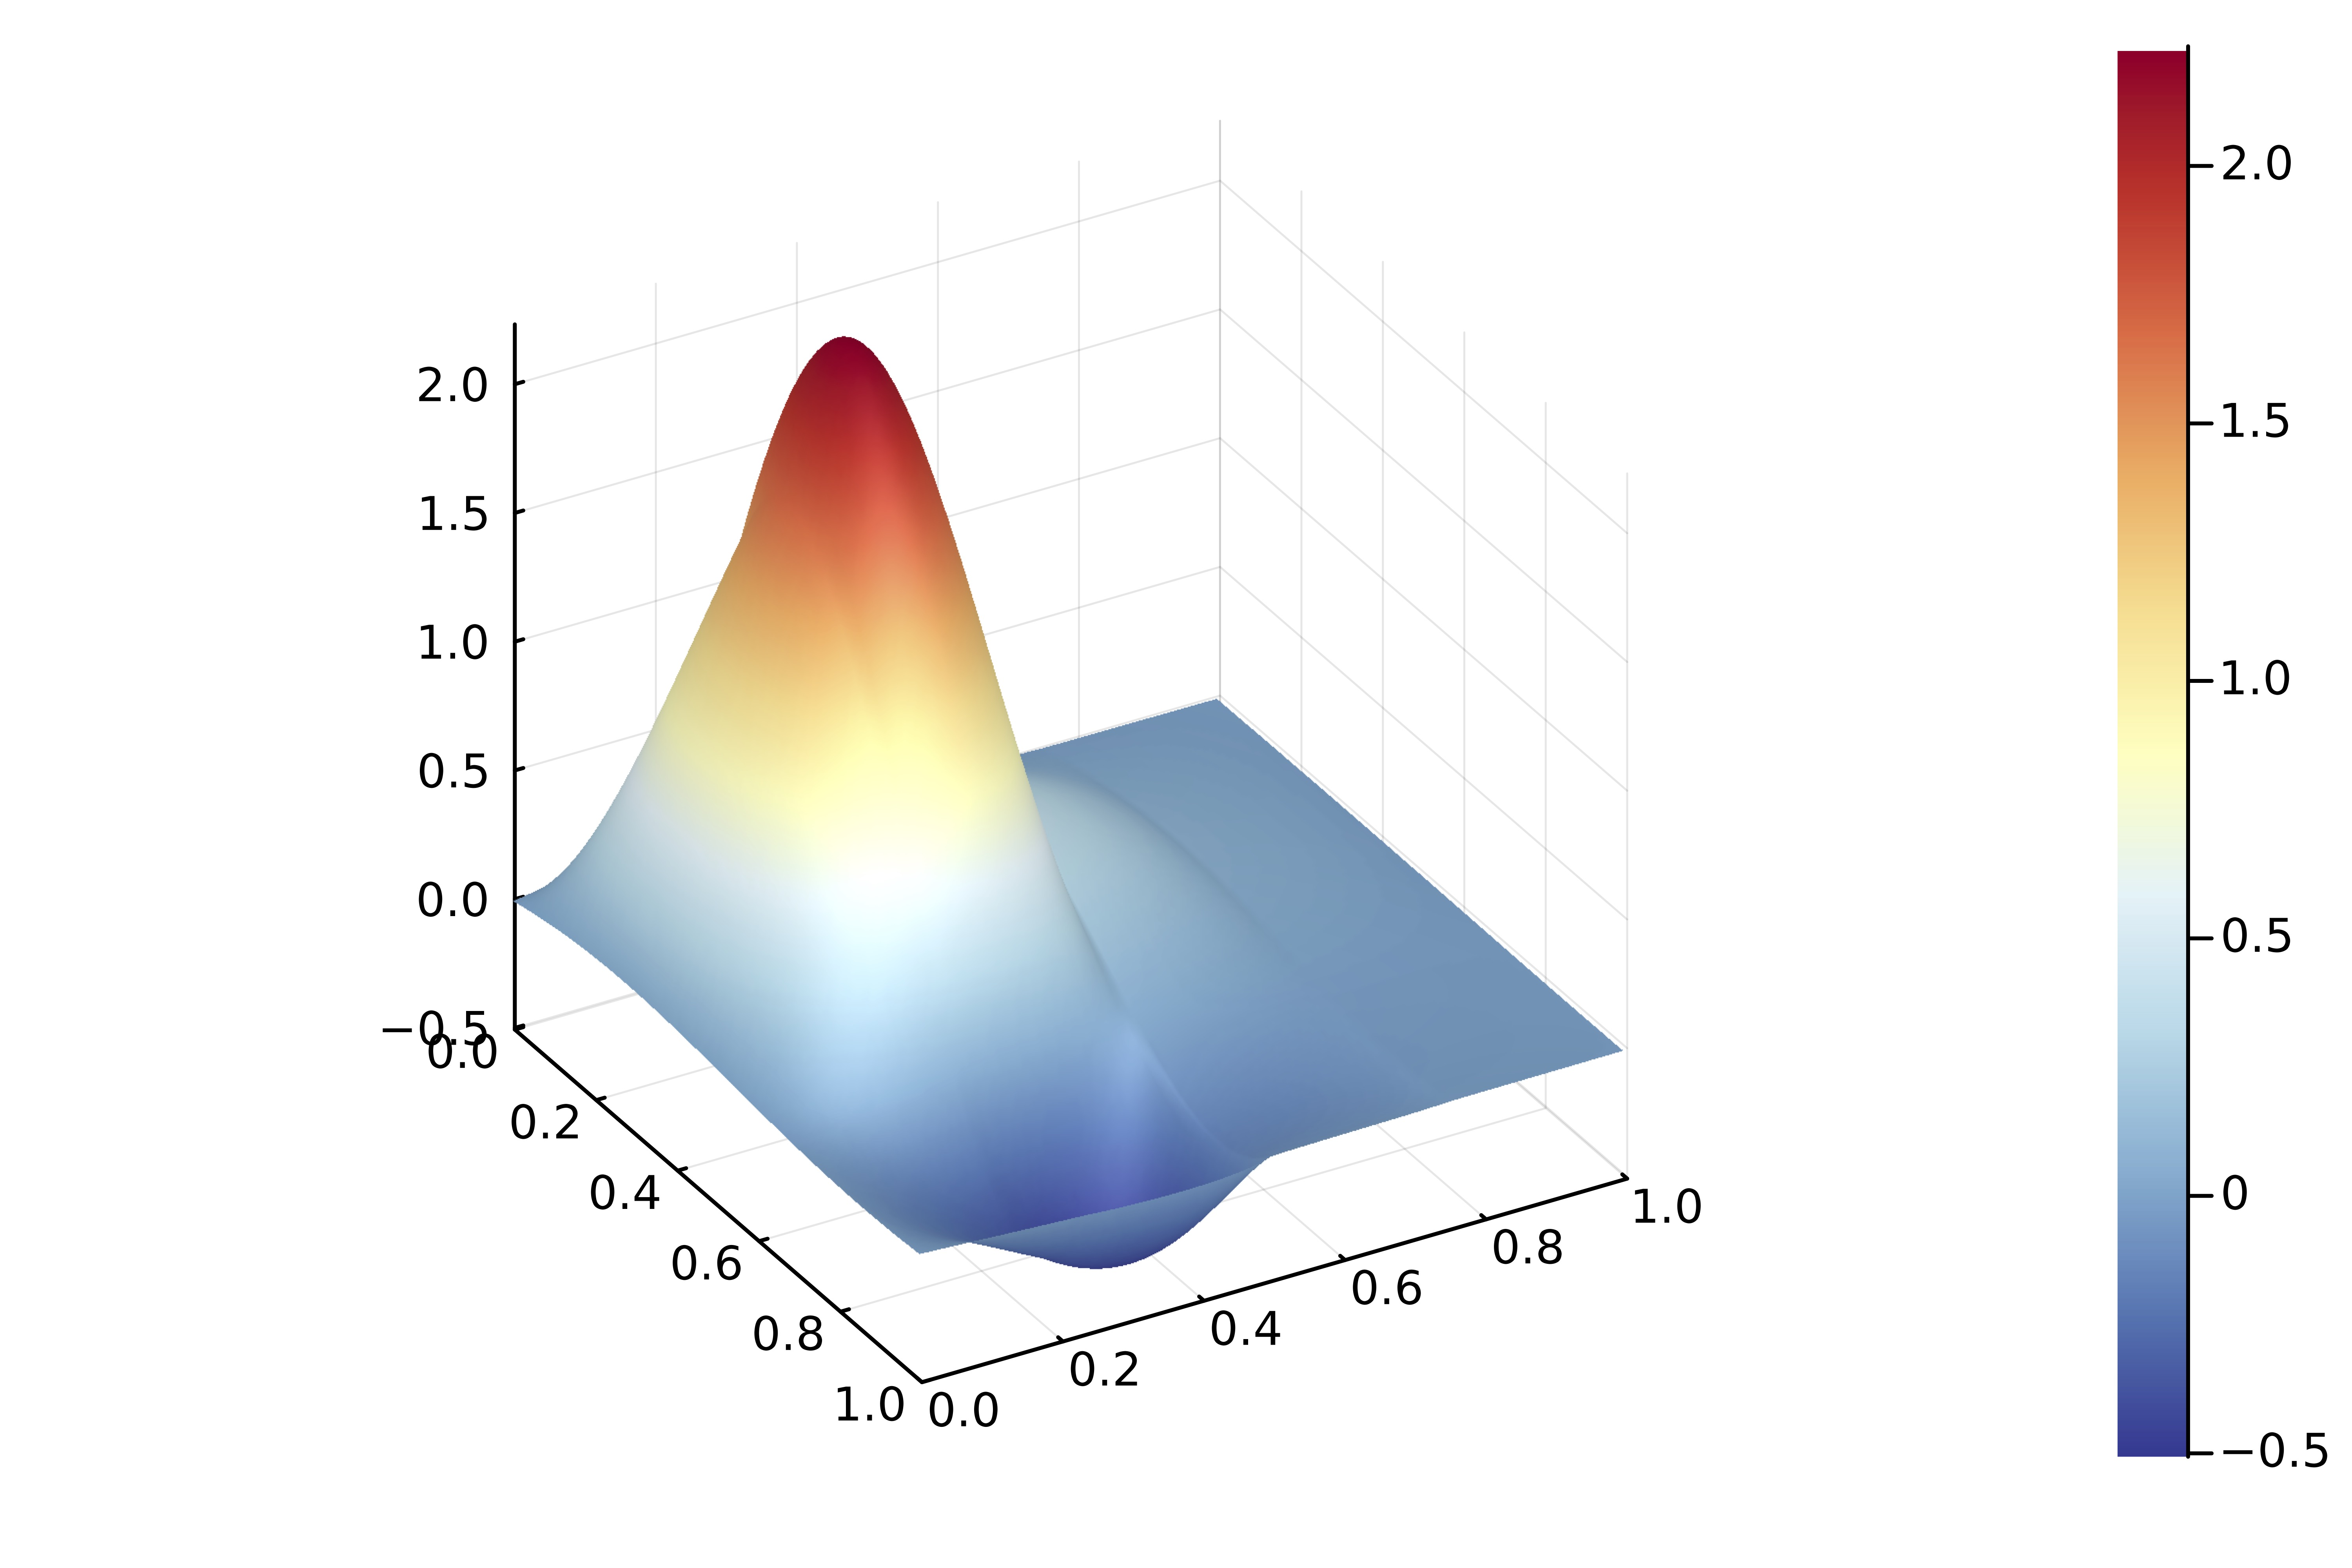
\includegraphics[width=0.25\linewidth]{figures/unc-state-1.jpg}}\qquad    
  \subfloat{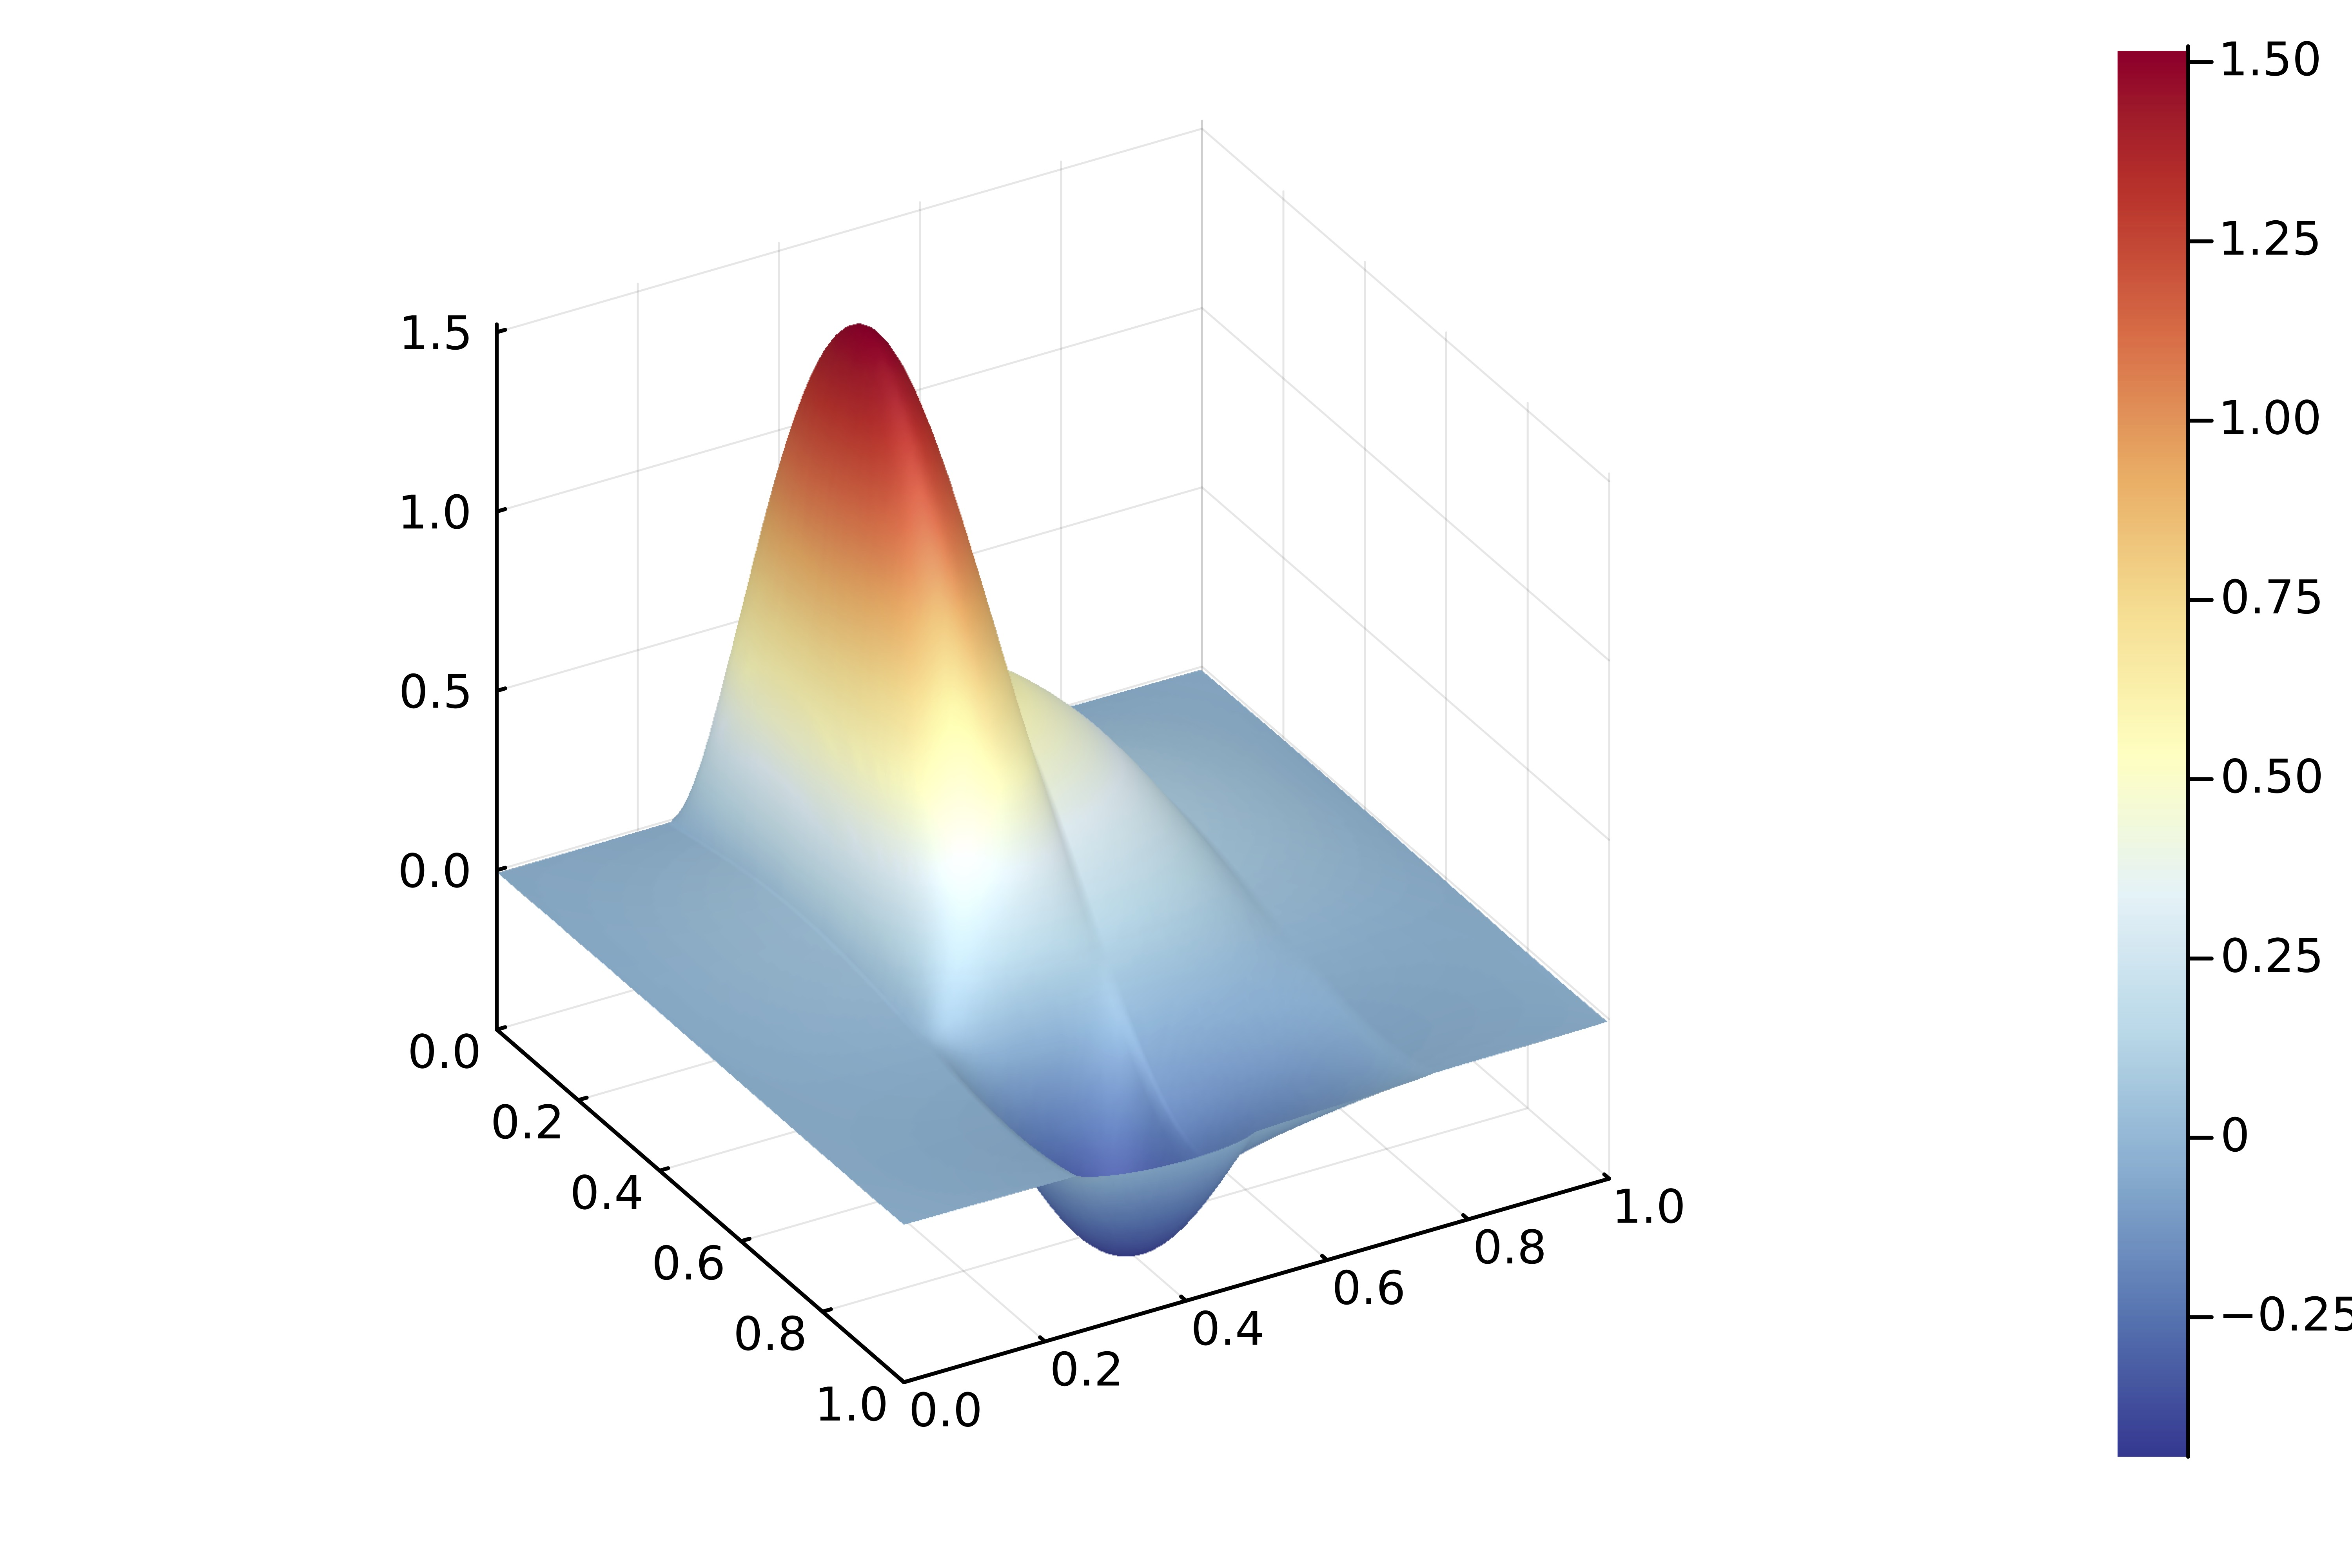
\includegraphics[width=0.25\linewidth]{figures/unc-state-2.jpg}}\qquad 
   \subfloat{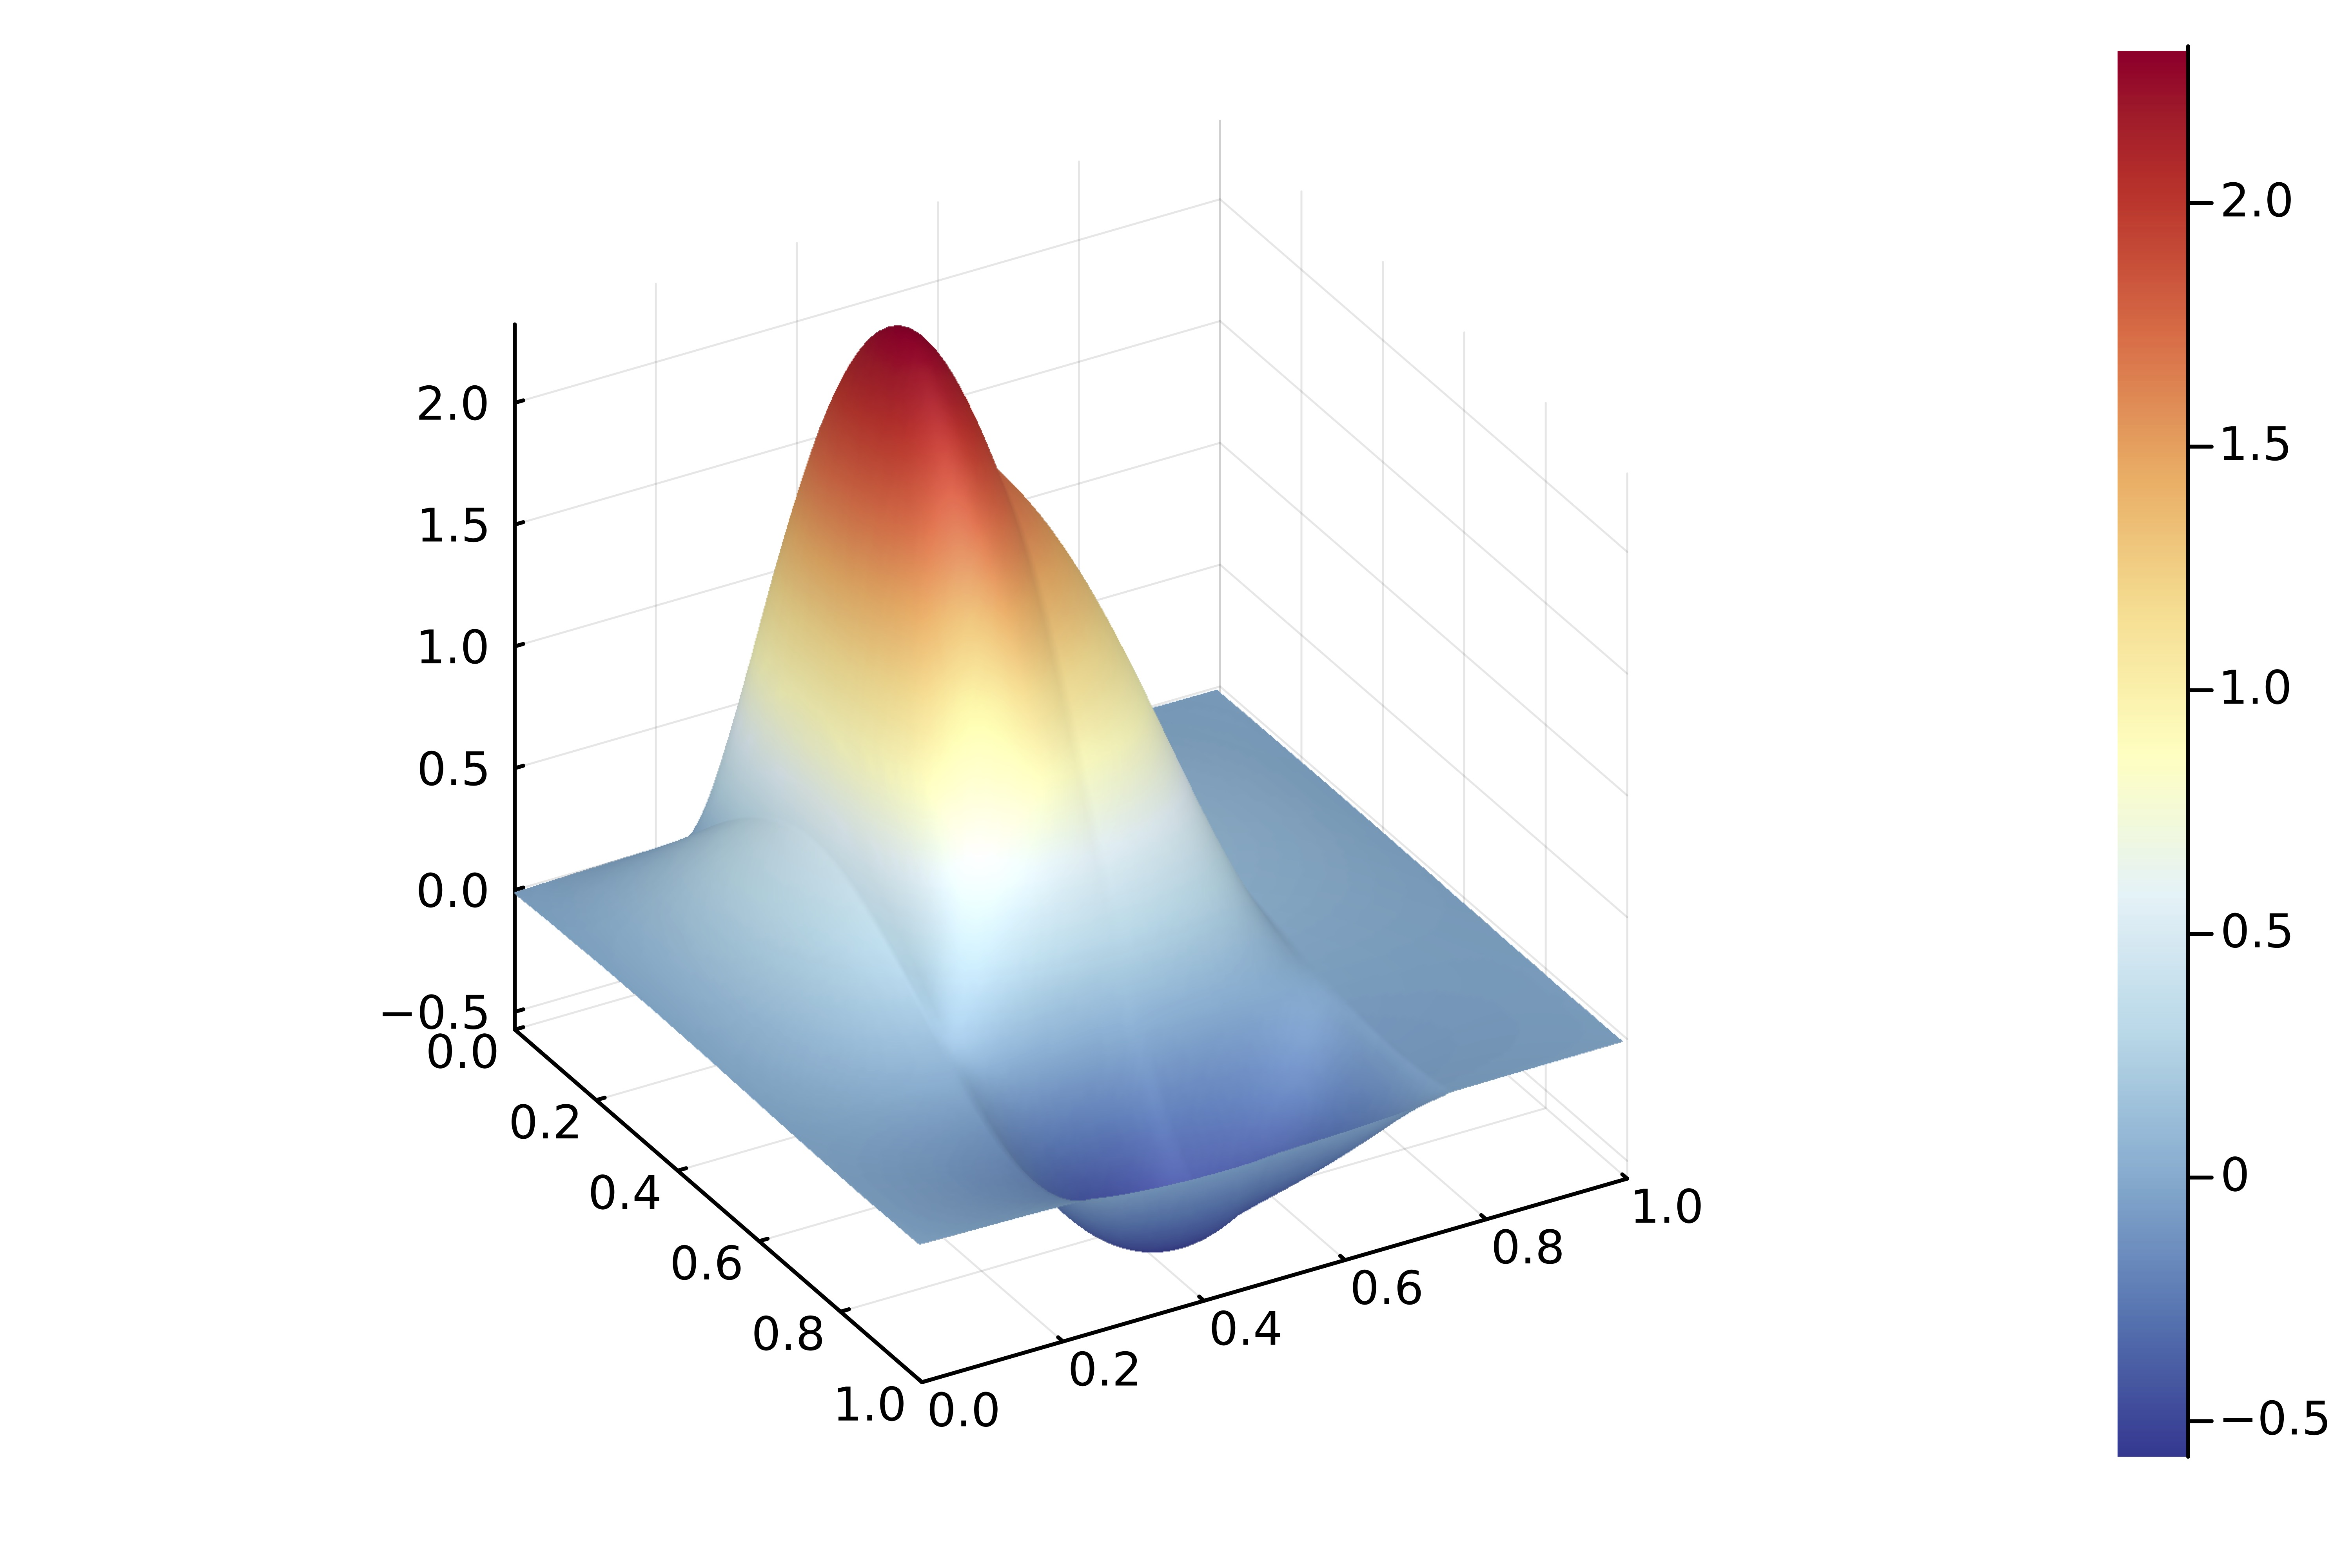
\includegraphics[width=0.25\linewidth]{figures/unc-state-3.jpg}}
\caption{Uncontrolled, random states: Three realizations of $u(\xi)$ computed by setting $z \equiv 0$ in \eqref{eq:rand_pde}.}
\label{fig:fig1}
\end{figure}
}
\end{frame}

\begin{frame}{Additional Assumptions}
    \begin{exampleblock}{}
        \begin{itemize}
            \item We again define
\begin{eqnarray}\nonumber
{\mathcal{J}}(u,z)&:=&\frac{1}{2}\int_{\Xi}\int_{D} 
|u(x,\xi) - \widetilde{u}(x)|^2\,dx\,dP(\xi) 
+ \frac{\alpha}{2} \int_{D} |z(x)|^2 \,dx% \\
% &=& \frac{1}{2} \E_{P}[\|u(\cdot) - \widetilde{u}\|^2_{H}] 
% + \frac{\alpha}{2} \| z \|^2_{H}
\label{object}
\end{eqnarray}
            \item $\alpha > 0$ and $\tilde{u} \equiv 1/2$. 
            \item The control constraints are taken to be
\[
Z_{\rm ad} := \left\{ v \in L^2(D) \left| -0.75 \le v \le 0.75 \text{ a.e. } D \right.\right\}.
\]
            \item These constants are merely for illustration. The algorithm is robust for wide ranges of parameters.
        \end{itemize}
    \end{exampleblock}
\end{frame}

\subsection{Generalizing Newton's Method}
\begin{frame}{Reformulation as Nonsmooth Equation}
    \begin{exampleblock}{}
        \begin{itemize}
            \item \visible<1->{We need to solve \alert{thousands of large constrained optimization problems.}}
            \item \visible<2->{The model class has favorable structure: The unique optimal solution $z$ satisfies the nonsmooth equation in $L^2(D)$\vspace{-1ex}
\begin{equation}\label{eq:proj-eq}
z - \mathrm{Proj}_{Z_{\rm ad}}(z - c(\mathbb E_{P}[\Lambda(z)] + \alpha z)) = 0.\vspace{-2ex}
\end{equation}
\item $c > 0$ constant, 
\item $\mathrm{Proj}_{Z_{\rm ad}}$ is the metric projection on $Z_{\rm ad}$,
\item $\Lambda(z)$ is the adjoint state mapping.}
\visible<3->{For fixed $\xi$, $\lambda(\xi) := \Lambda(z,\xi)$ satisfies
\[
\aligned
\lambda(\xi) &= A^{-*}(\xi)(-\mathcal{J}'_u(A^{-1}(\xi)(z+g(\xi)),z))
             = -A^{-1}(\xi)(A^{-1}(\xi)(z+g(\xi)) - \tilde{u}).
\endaligned
\]}\visible<4->{
 Under the standing assumptions, we can rewrite \eqref{eq:proj-eq} as
\begin{equation}\label{eq:nse}
\mathcal{F}(z) := z - \min\left\{0.75,\max\left\{-0.75,z- c(\mathbb E_{P}[\Lambda(z)]+\alpha z)\right\}\right\} = 0.
\end{equation}\vspace{-2ex}
}
        \end{itemize}
    \end{exampleblock}
\end{frame}

\begin{frame}{The Semismooth Newton Method}
    \begin{exampleblock}{}
        \begin{itemize}
            \item A popular method for structured PDE-constrained optimization problems (Hinterm\"uller, Ito, Kunisch (2002), M.~Ulbrich (2002))
            \item \visible<2->{
            $\mathcal{F}$ needs to be \alert{Newton differentiable} on an open neighborhood of that solution.}
            \item \visible<3->{
            This necessitates the existence 
            of a family of bounded linear operators $\mathcal{G}$, uniformly bounded on a neighborhood of the solution that fulfill
            \[
            \mathcal{F}(z + h) - \mathcal{F}(z) - \mathcal{G}(z + h)h = o(\|h\|).
            \]\vspace{-2ex}
            }
            \item \visible<4->{
            $\mathcal{G}$ is called a \alert{Newton derivative}.} 
            \item \visible<5->{For operators generated by the \alert{nonsmooth} functions $\max\{0,x\}$, $\min\{0,x\}$ we typically need a \alert{norm gap} in order to get the previous approximation property.
            }
        \end{itemize}
    \end{exampleblock}
\end{frame}

\begin{frame}{Computing Newton Derivatives}
    \begin{exampleblock}{}
        \begin{itemize}
            \item 
            \visible<1->{\alert{Regularity} of the individual adjoint equations ($\xi$-dependent, deterministic) leads to showing that $\mathbb E_{P}[\Lambda(\cdot)]$ is \alert{smooth from $L^2(D)$ into $L^p(D)$ with $p > 2$}.
            }
            \item 
            \visible<2->{
            Taking $c = \alpha^{-1}$, we can remove $z$ from inside the projection operator
            }
            \item 
            \visible<3->{
            The \alert{elliptic regularity} then allows us to demonstrate the necessary \alert{norm gap} and leads to \alert{Newton differentiability} of $\mathcal{F}$ using the family of maps} 
            \visible<4->{
            \[
[\mathcal{G}(z)\delta z](x) 
= 
\left
\{\begin{array}{cc}
\delta z(x)& \text{ if } z(x) - c(\mathbb E_{P}[\Lambda(z)](x) + \alpha z(x)) > 0.75\\
\delta z(x)& \text{ if } z(x) - c(\mathbb E_{P}[\Lambda(z)](x) + \alpha z(x)) < -0.75\\
c(\mathbb E_{P}[\Lambda'(z)\delta z] + \alpha \delta z)& \text{ else.}
\end{array}
\right.
\]
}
            \item 
            \visible<5->{Given $z_k \in L^2(D)$ with $\|\mathcal{F}(z_k)\|_{L^2} \ne 0$, the step calculation amounts to finding $\delta z \in L^2(D)$:
\[
\mathcal{G}(z_k)\delta z = - \mathcal{F}(z_k).
\]
}
        \end{itemize}
        \vspace{-4ex}
    \end{exampleblock}
\end{frame}

\begin{frame}{SSN as Primal-Dual Active Set Method}
    \begin{exampleblock}{}
        \begin{itemize}
            \item \visible<1->{\alert{ACHTUNG:} We only implicitly know the generalized Jacobian of $\mathcal{F}$! Need \alert{iterative solvers}.}
        \end{itemize}
        \begin{enumerate}
    \item \visible<2->{\textbf{Estimate} Given $z_k \in L^2(D)$ such that $\|\mathcal{F}(z_k)\|_{L^2} > 0$ compute 
    \[
    \aligned
    \mathcal{A}^1_k &:= \left\{x \in D \left| z_k(x) - c(\mathbb E_{P}[\Lambda(z)](x) + \alpha z_k(x)) > 3/4 \right. \right\}\\
    \mathcal{A}^2_k &:= \left\{x \in D \left| z_k(x) - c(\mathbb E_{P}[\Lambda(z)](x) + \alpha z_k(x)) < -3/4 \right. \right\}\\
    \mathcal{I}_k &:= D \setminus (\mathcal{A}^1_k \cup \mathcal{A}^2_k)
    \endaligned
    \]\vspace{-2ex}
    }
    \item \visible<3->{\textbf{Reduce} Set 
    % \[
    % \aligned
    $
    \delta z_k := 3/4 - z_k  \text{ on } \mathcal{A}^1_k,\;
    \delta z_k := -3/4 - z_k \text{ on } \mathcal{A}^2_k.
    $
    % \endaligned
    % \]
    }
    \item \visible<4->{\textbf{Solve} for $\delta z_k|_{\mathcal{I}_k}$:
    \[
    \mathbb E_{P}[\Lambda'(z_k)\delta z|_{\mathcal{I}_k}]|_{\mathcal{I}_k}  + \alpha \delta z|_{\mathcal{I}_k} = 
    -[\mathbb E_{P}[\Lambda(z_k)] + \alpha z_k]|_{\mathcal{I}_k} 
    - [\mathbb E_{P}[\Lambda'(z_k)\delta z|_{\mathcal{A}^1_k\cup \mathcal{A}^2_k}]|_{\mathcal{I}_k} 
    \]\vspace{-2ex}
    }
    \item \visible<5->{\textbf{Update} $z_{k+1} := z_k + t_k\delta z_k$ for some damping factor $t_k > 0$ (e.g. $t_k = 1$).
    }
\end{enumerate}
    \end{exampleblock}
\end{frame}

\section{Computational Statistics}
\subsection{Experimental Rates of Convergence}
\begin{frame}\frametitle{Details of the Implementation}
\begin{exampleblock}{}
\begin{itemize}
    \item Implemented in Julia  \cite{Julia-2017} using the FE package Gridap \cite{Badia2020} on Simula's eX3 computer\footnote{\tiny
    Experimental Infrastructure for the Exploration of Exascale Computing (eX3), supported by the Research Council of Norway under contract No. 270053}
    \item Multithreading is essential for efficiency. Julia can handle this easily.
    \item State, adjoint, and sensitivity equations for separate samples $\xi_i$ do not communicate.
    \item Hessian-vector products detailed earlier, see e.g. \cite[Chap. 1.6.5]{HPUU09}.
    \begin{center}
        \textbf{This is how OUU algorithms using Hessians compete with cheap iteration cost in first-order methods.}
    \end{center}\pause
    \item  Iterations reuse the $n$ random stiffness matrices (state, adjoint, hess-vec); prefactor, cache. 
     \item Use standard CG algorithm for iterative scheme \cite{MRHestenes_EStiefel_1952}. 
      \item $c = 10^{-3}$ (scaling factor for active and inactive sets), damping factor $t_k = 1.00$. 
      \item Stopping criterion: absolute, relative tolerance of $10^{-8}$ for the discrete $L^2$-norm of $\mathcal{F}(z_k)$.
      \item After +100K runs with random data, SSN converges in less than 10 iterations on average.
\end{itemize}    
\end{exampleblock}
\end{frame}

\begin{frame}{Example}
\begin{figure}
\subfloat{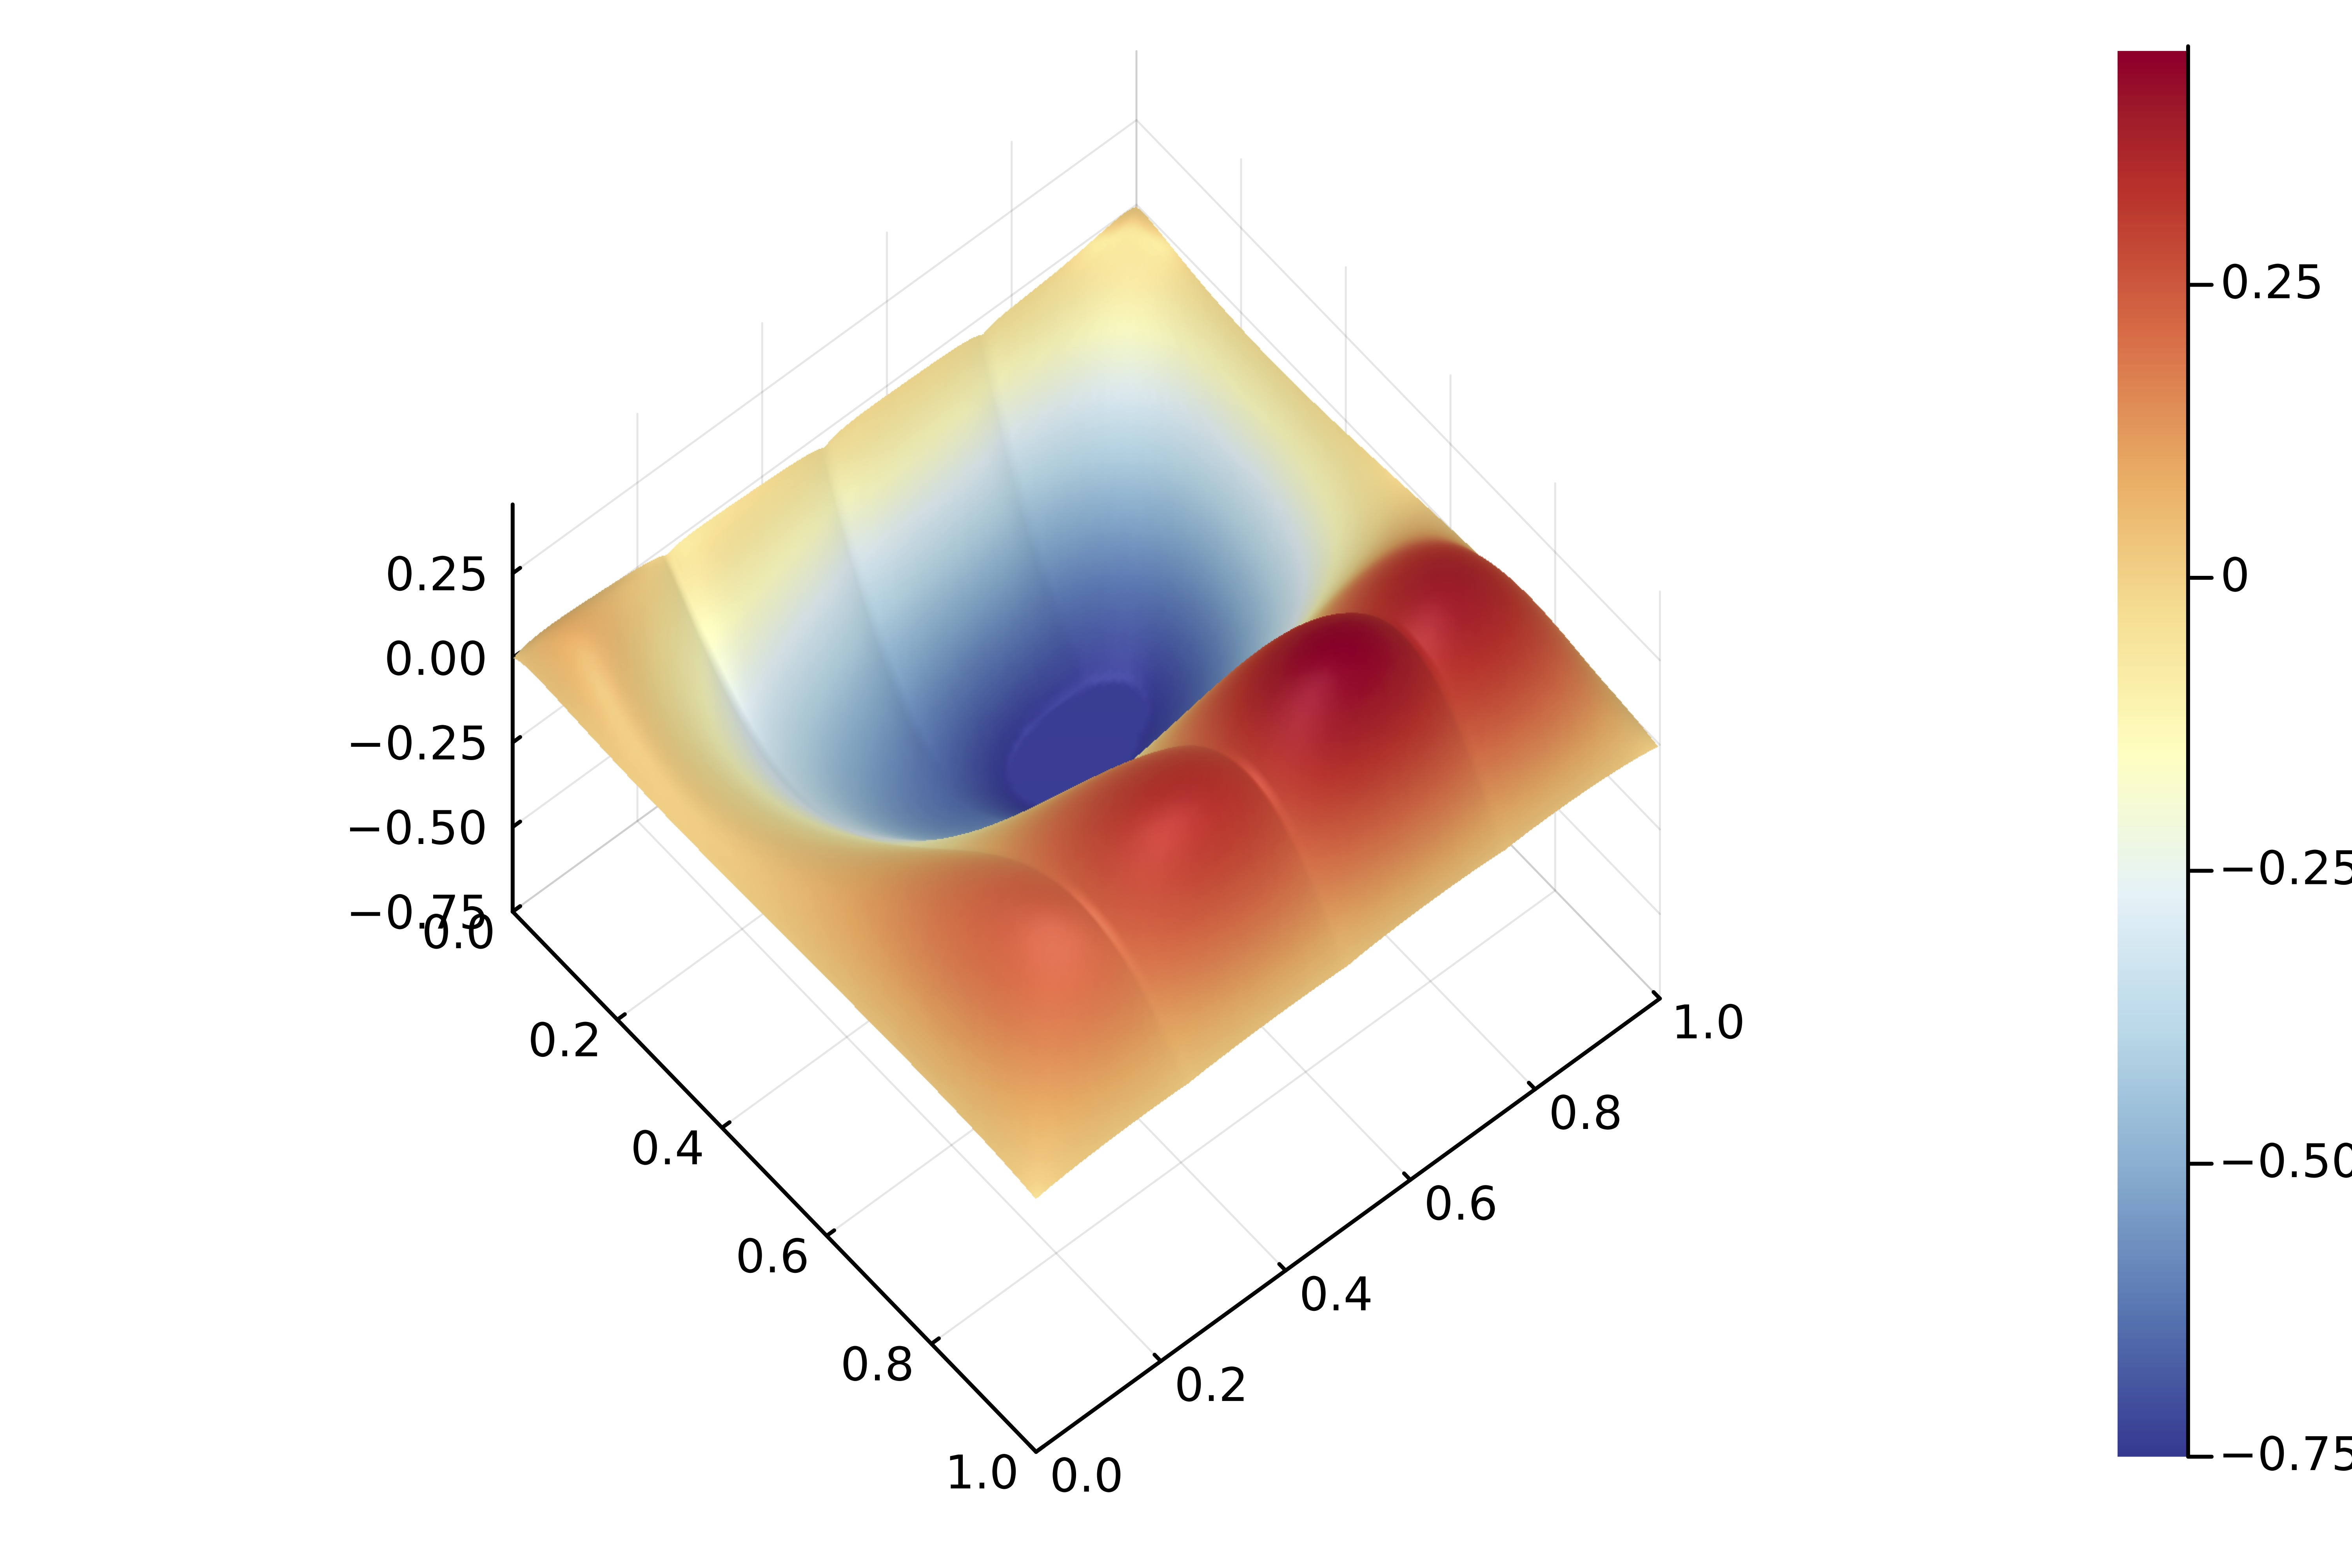
\includegraphics[width=0.4\linewidth]{Part II/figures/opt-ctrl-z-500.jpg}}\qquad   \subfloat{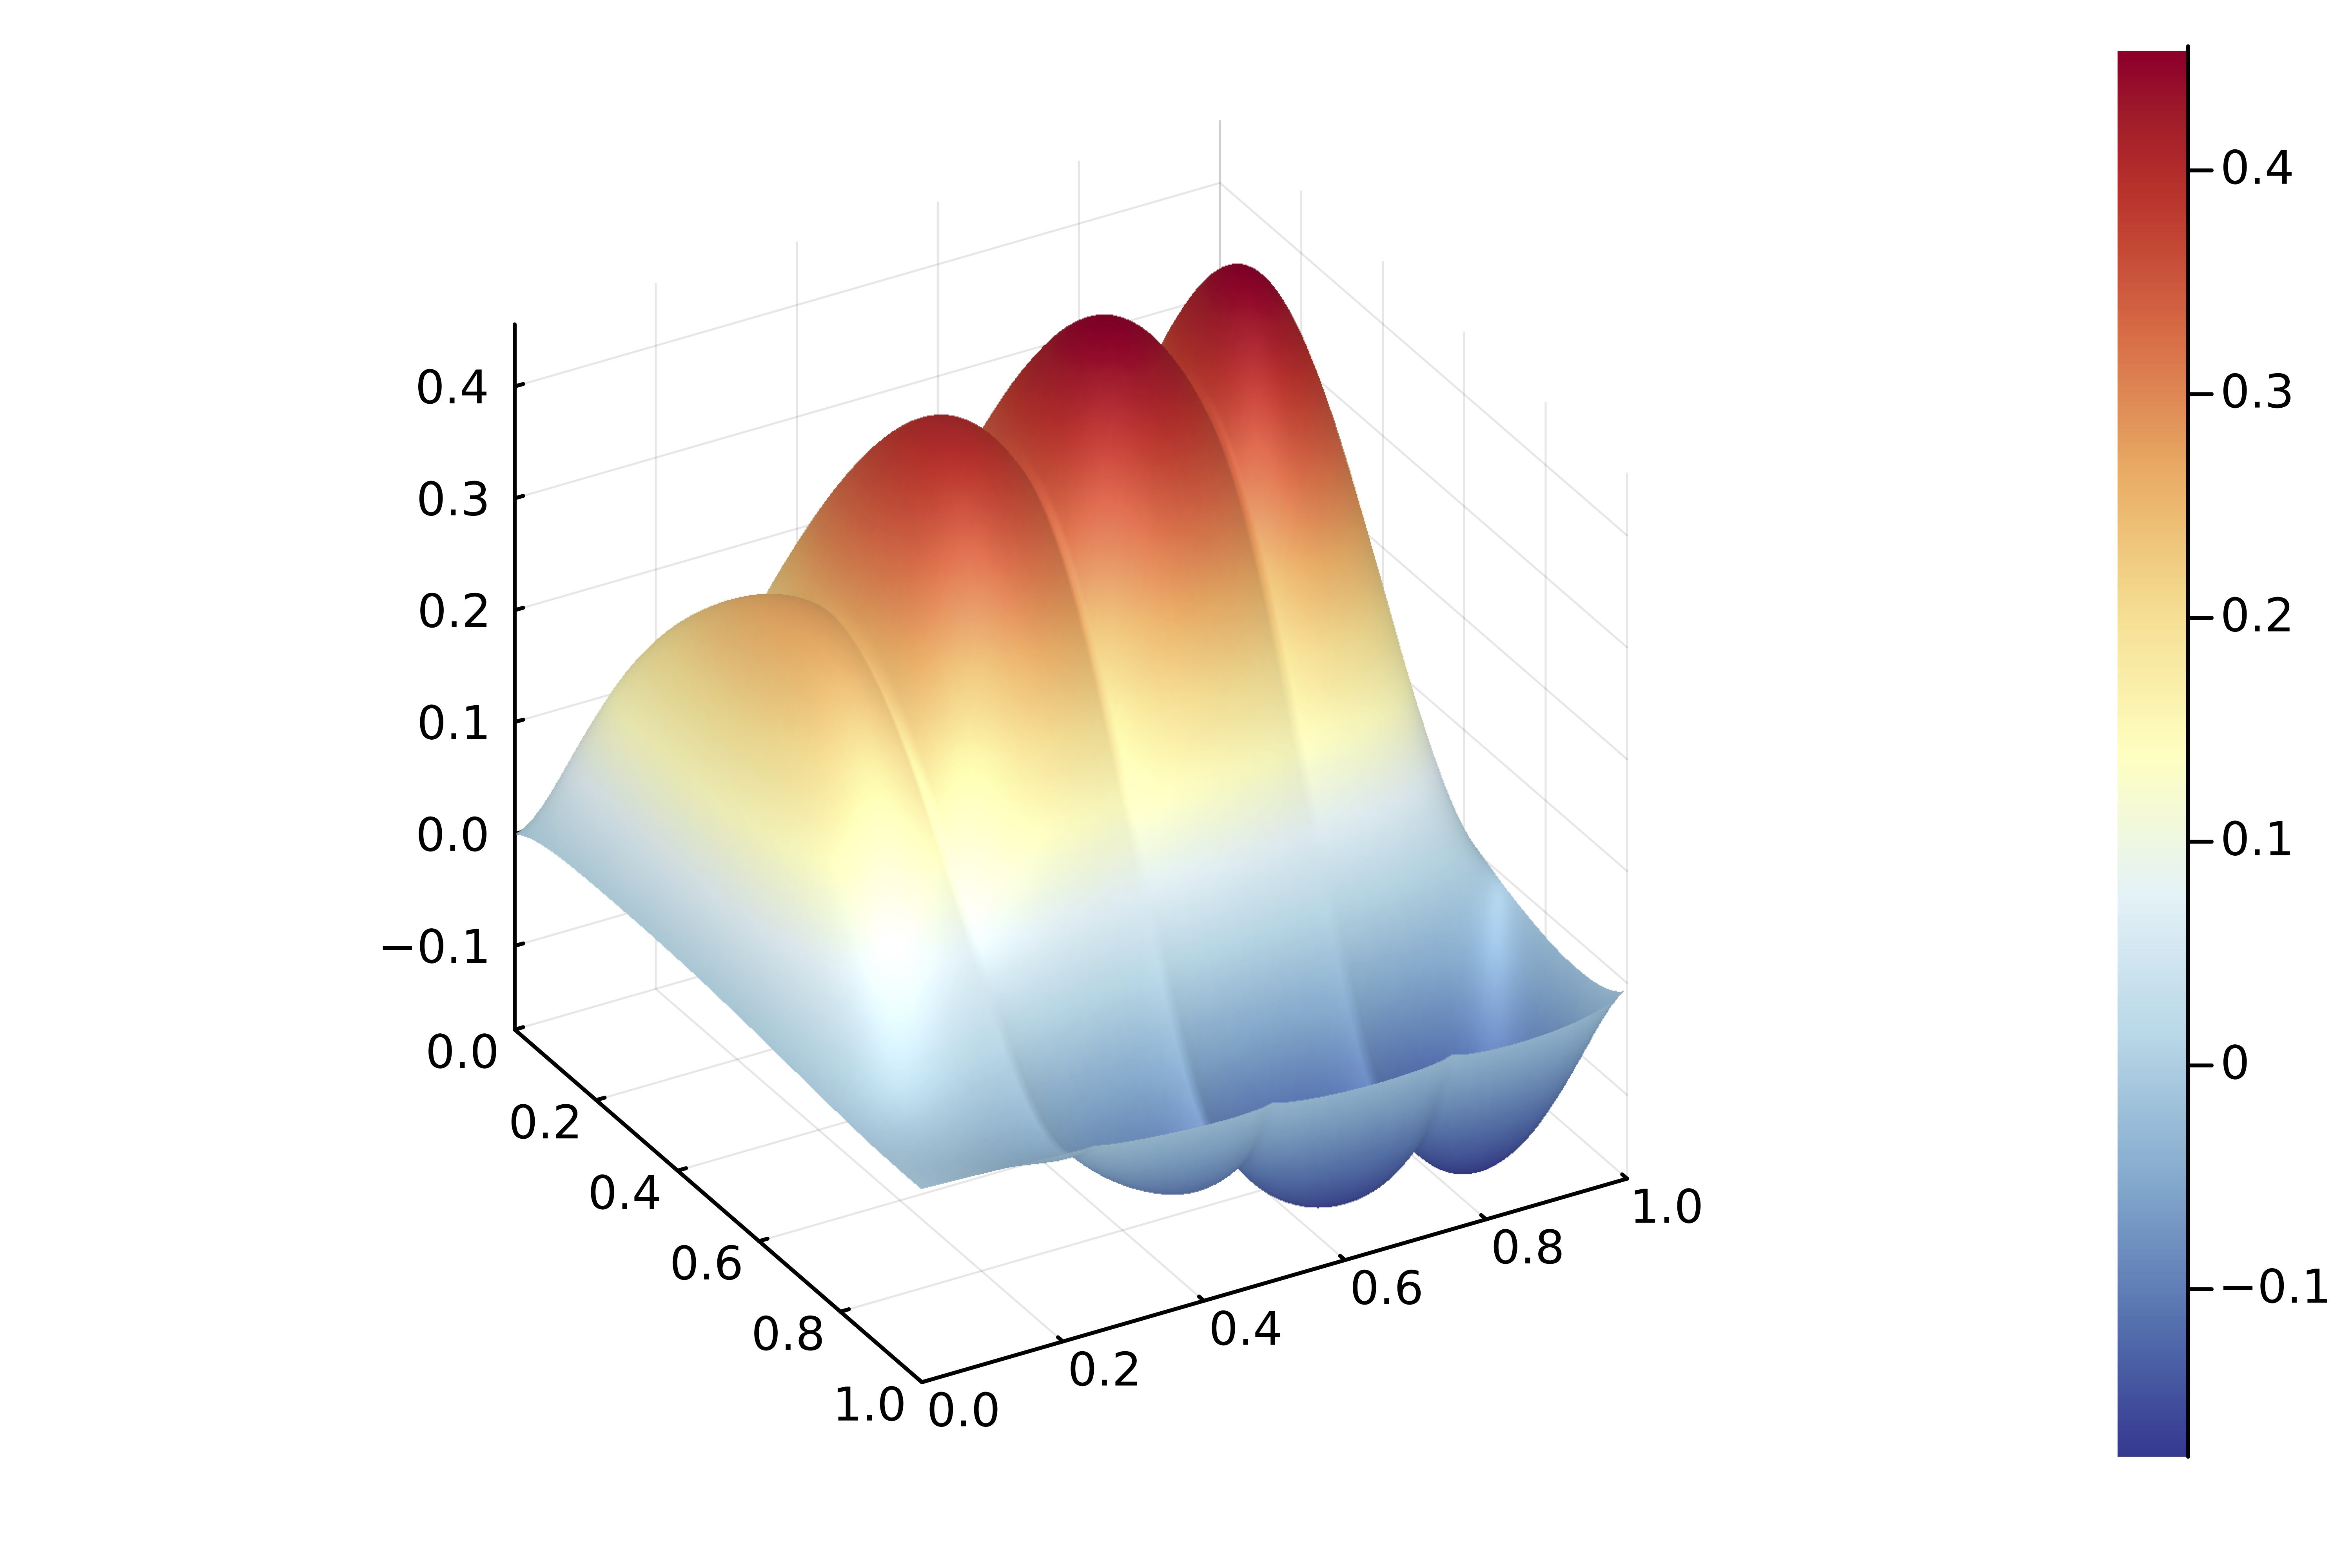
\includegraphics[width=0.4\linewidth]{Part II/figures/avg-ctrld-state-500.jpg}}\qquad 
\caption{Optimal solution and average states:\\ 
(left) the optimal control computed for a sample of size $n = 500$ on a uniform mesh with 16129 degrees of freedom.\\ 
(right) the effect of $z(P_n)$ on the state variables $u(\xi)$ out of sample; displayed: $\frac{1}{n}\sum_{i=1}^{n} A(\xi_i)^{-1}(z(P_n) + g(\xi_i))$.
\label{fig:fig2}}
\end{figure}
\end{frame}

\begin{frame}\frametitle{Setting up the Experiment}
\begin{exampleblock}{}
    \begin{itemize}
        \item \textbf{``True'' solution:} Fix a mesh $900$ DoFs, solve to high accuracy using $n = 500$
        \item  This yields a ``true'' solution $z(P_n)$ and optimal value $v(P_n)$. 
        \item Select smaller sample sizes $m = 1,\dots,M$, with $M = 100$, resolve to obtain $z(P_m)$ and $v(P_m)$.
        \item For each $m$, repeat experiment 100 times and generate a sample of solutions and optimal values \[
        \left\{(z(P_{m,j}),v(P_{m,j})\right\}_{j=1}^{100}
        \]
        \item \textbf{We do not subsample the data used to compute  $z(P_n)$ and $v(P_n)$.}
        \item Compute and save  
        \[
        \|z(P_{m,j}) - z(P_n)\|_{L^2}
        \text{ and }
        |v(P_{m,j}) - v(P_n)|.
        \]
    \end{itemize}
\end{exampleblock}
\end{frame}

\begin{frame}\frametitle{Results}
\begin{figure}
\subfloat{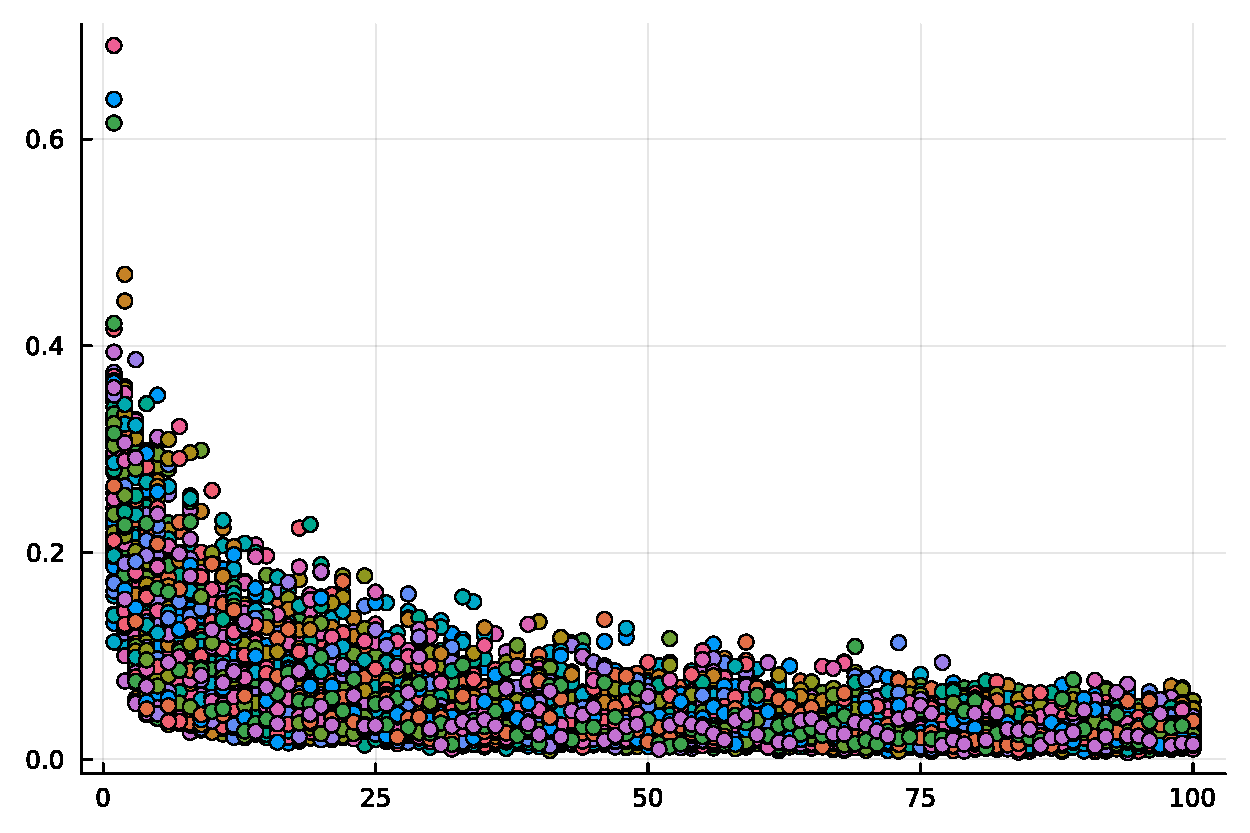
\includegraphics[width=0.25\linewidth]{Part II/figures/empirical-stab-opt-ctrl.pdf}}\qquad
\subfloat{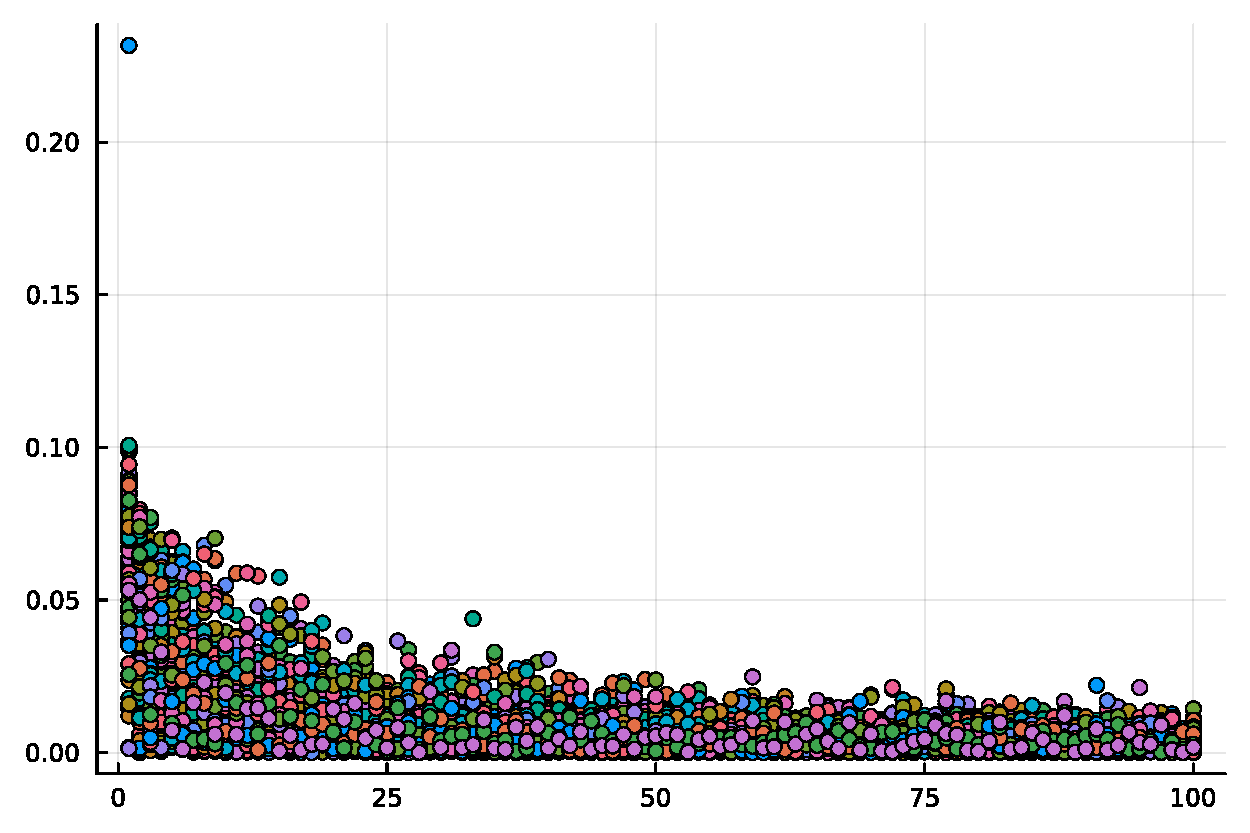
\includegraphics[width=0.25\linewidth]{Part II/figures/empirical-stab-opt-values.pdf}}
\caption{Experimental convergence rates of the optimal solutions and optimal values:  subsamples $m$ versus 100 instances of
(left) $\|z(P_m) - z(P_n)\|_{L^2(\Omega)}$ and
(right) $|v(P_m) - v(P_n)|$ for $m = 1,\dots,100$
\label{fig:fig3}}
\end{figure}
\begin{exampleblock}{}
    \begin{itemize}
        \item Use simple regression technique to compute
        \[
        \|z(P_m) - z(P_n)\|_{L^2(\Omega)} \in O(m^{-0.53656})
        \text{ and }
        |v(P_m) - v(P_n)| \in O(m^{-0.66035})
        \]
        \item \textbf{Keep in mind:} There is FE approximation error, sampling error, floating point error, quadrature error, inexact solution tolerance for Newton and CG! 
    \end{itemize}    
\end{exampleblock}
\end{frame}

\subsection{Subsampling Bootstrapped Confidence Intervals}
\begin{frame}{Return to the CLT}
    \begin{exampleblock}{}
        \begin{itemize}
            \item We saw that a CLT holds for the optimal values:
            \[
            \sqrt{n}(v(P_{n})-v(P)) \rightsquigarrow \mathcal{N}(0,P(f(z(P)))^2).
            \]
            \item But $v(P)$ and $P(f(z(P)))^2$ are \alert{almost never available.}
            \item Is this a \textbf{useless} statement? \textbf{No, why not?}
        \end{itemize}
    \end{exampleblock}
\end{frame}

\begin{frame}{Bootstrapping and Subsampling}
    \begin{exampleblock}{}
        \begin{itemize}
            \item \visible<1->{Traditional bootstrap: Use samples of size $n$ with replacement from $\{1,\cdots,n\}$ \cite[]. The \textbf{``right''} sample size, but the \textbf{``wrong''} distribution.
            \item Might not be consistent, for our purpose very time consuming as $n \to +\infty$.
            }
            \item \visible<2->{Subsampled bootstrap: Use samples of size $b \ll n$ without replacement from $\{1,\dots,n\}$. The \textbf{``wrong''} sample size, but the \textbf{``right''} distribution.}
            \item \visible<3->{Fix $n \in \mathbb N$, let $\xi_{1},\ldots,\xi_{n}$ be an iid sample from $P$. 
            \item Choose $b \ll n$ and draw new sample from $\xi_{n_1},...,\xi_{n_b}$ 
from $\{1,...,n\}$ with cardinality $b$. Define 
            \[
P^*(n_1,...,n_b)=\frac{1}{b}\sum_{i=1}^{b}
\delta_{\xi_{n_i}} \text{ and associated optimal value } v(P^*(n_1,...,n_b)).
\]}
            \item \visible<3->{This subsampling based bootstrap will allow us to estimate the empirical process $\sqrt{n}(v(P_n)(\cdot) - v(P))$ provided $n,b \to +\infty$, $b/n \to 0$
            }
        \end{itemize}
    \end{exampleblock}
\end{frame}
    
\begin{frame}{Subsampling Bootstrap}
    \begin{exampleblock}{}
        \begin{itemize}
            \item \visible<1->{\textbf{Three indices} $n$ (original sample size), $b \ll n$ (subsample size), $m$ (number of random samples of size $b$).
            \item Define $N_j^{n,b}\subset\{1,...,n\}$ be randomly chosen 
with cardinality $\#N_j^{n,b}=b$ for $j=1,...,m$. }
            \item \visible<2->{
             $P_n^*(N_j^{n,b})$ denotes empirical 
            measure based on $\{\xi_i : i\in N_j^{n,b}\}$.
            \item $ v(P_n^*(N_j^{n,b}))$ is the associated optimal value.
            \item Need $n,b,m \to +\infty$, $b/n \to 0$.
            }
        \end{itemize}
    \end{exampleblock}
    \visible<3->{
    \begin{exampleblock}{}
        \begin{itemize}
            \item \textbf{Observe:} \vspace{-2ex}
\[
\aligned
-\sqrt{b}(v(P_{n})-v(P)) 
&= 
-\frac{\sqrt{b}}{\sqrt{n}}(\sqrt{n}(v(P_{n})-v(P))) \rightsquigarrow 0,\\
\sqrt{b}(v(P_n^*(N_j^{n,b}))-v(P_{n})) &= 
\sqrt{b}(v(P_n^*(N_j^{n,b}))-v(P))-\sqrt{b}(v(P_n)-v(P))\\
\only<4>{
\sqrt{b}(v(P_n^*(N_j^{n,b}))-v(P_{n}))
 &\rightsquigarrow \mathcal{N}(0,P(f(z(P)))^2)
 }
\endaligned
\]
\end{itemize}
\end{exampleblock}
}
\end{frame}

\begin{frame}{Interpretation}
    \begin{exampleblock}{}
        \begin{itemize}
            \item \visible<1->{So what does $\sqrt{b}(v(P_n^*(N_j^{n,b}))-v(P_{n}))
 \rightsquigarrow \mathcal{N}(0,P(f(z(P)))^2)$
            \textbf{actually mean for us?}}
            \item \visible<2->{First off: we can actually \textbf{compute} $v(P_n^*(N_j^{n,b}))$ and $v(P_{n})$.}
            \item \visible<3->{If $L_{n,b}(\cdot)$ is the empirical cumulative distribution function for $\sqrt{b}(v(P_n^*(N_j^{n,b}))-v(P_{n}))$, we can argue that 
            \[
L_{n,b}^{-1}(\alpha/2) < \sqrt{n}(v(P_{n})-v(P)) < L_{n,b}^{-1}(1-\alpha/2),
\]
holds with probability close to $1-\alpha$.}
            \item \visible<4->{
            Consequently, we can compute $1-\alpha$ \textbf{confidence intervals} on the \textbf{unattainable optimal value} $v(P)$ by 
            \[
\aligned
\overline{c}_{n,b,\alpha} &= v(P_{n}) - n^{-1/2}L^{-1}_{n,b}(\alpha/2) \\
\underline{c}_{n,b,\alpha} &= v(P_{n})-n^{-1/2}L^{-1}_{n,b}(1-\alpha/2).
\endaligned
\]
            }
        \end{itemize}
        
    \end{exampleblock}
\end{frame}

\begin{frame}{Running the Experiment}
    \begin{exampleblock}{}
    \begin{minipage}{0.6\textwidth}
\begin{itemize}
            \item \visible<1->{
            Asymptotic theory requires a significant amount of computational power.
            }
            \item \visible<2->{
8-10 semismooth Newton steps means  \alert{several million PDE solves}.
            }
            \item \visible<3->{
             Thus, we use a coarse mesh size: 32 $\times$ 32. 
             \item $n=2000$, $b=1000$, $m=1000$.
             \item confidence level $95$ ($\alpha = 0.05$ in the preceding computation).}
             \item \visible<4->{This yields
\[
\underline{c}_{n,b,\alpha} = 0.089148 \text{ and } \overline{c}_{n,b,\alpha} = 0.090720.
\]
            }
        \end{itemize}
    \end{minipage}%
     \begin{minipage}{0.4\textwidth}
         \visible<4->{
    \begin{figure}
  \centering
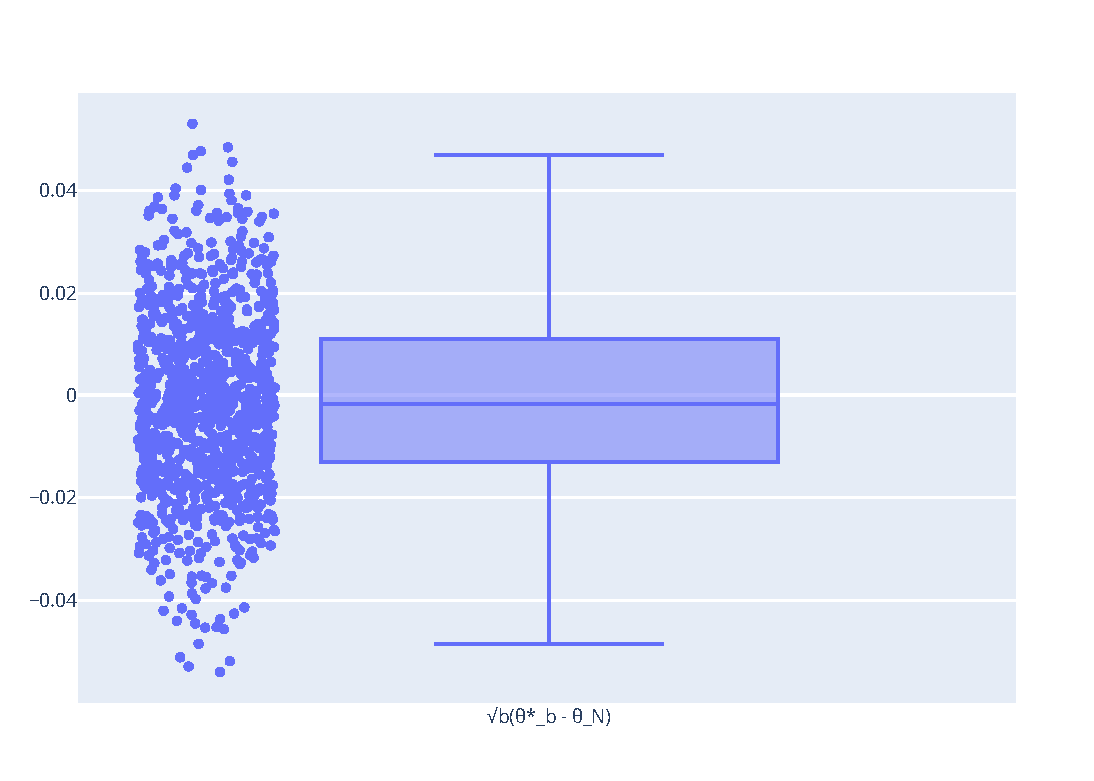
\includegraphics[width=\linewidth,keepaspectratio]{Part II/figures/central-limit-2000-1000-1000-32-32.pdf}
\caption{Subsampling bootstrapped 95\% confidence interval estimation.}
  % \caption{Box plot for the subsampling bootstrapped statistic $\sqrt{b}(v(P_n^*(N_j^{n,b}))-v(P_{n}))$ for a  mesh of size 32 $\times$ 32 using $n=2000$, $b=1000$ $j = 1,\dots,m$ with $m=1000$, $\alpha = 0.05$.} 
  \label{fig:clt}
\end{figure}%
    }
     \end{minipage}   
    \end{exampleblock}
\end{frame}

\begin{frame}{Discussion}
    \begin{exampleblock}{}
        \begin{itemize}
            \item \visible<1->{
            A 95\% confidence interval means that if we repeat this experiment 100 times, then 95 out of 100 times, the optimal value we compute for a sample of size $n = 2000$ should fall between $0.089148$ and $0.090720$.
            }
            \item \visible<2->{
            We tested this, too but got 84 out of 100.
            }
            \item \visible<3->{
            \alert{OPEN PROBLEM I}: Further experiments showed a relationship between $n, b, m$ and $h$ for this ``hit-or-miss'' statistic. A deeper study of this relationship would be interesting.
            }
            \item \visible<4->{
            \alert{OPEN PROBLEM II}: What can we derive for nonconvex risk-neutral or nonsmooth (possibly nonconvex) risk-averse problems? 
            }
        \end{itemize}
    \end{exampleblock}
\end{frame}

% \section{The Primal Dual Risk Minimization Algorithm}
% \subsection{Derivation}
% \subsection{Convergence Theory}

% \section{Implementation and Further Numerical Experiments}
% \subsection{Aspects of Implementation}
% \subsection{Examples}

\section{Summary and Outlook}


\end{document}